\documentclass[a4paper,oneside]{report}

%%%%%%%%%%%%%%%%%%%%%%%
%%% Préambule cours %%%
%%%%%%%%%%%%%%%%%%%%%%%

\usepackage[utf8]{inputenc}
\usepackage[T1]{fontenc}

\usepackage[frenchb]{babel}

\usepackage{amsmath}
\usepackage{xcolor}
\usepackage{graphicx}
\graphicspath{{Images/}}
\usepackage{color}
\usepackage{eurosym}
\usepackage{hyperref}
\usepackage{listings}	%code
\usepackage{color}
\lstset{
  language=Python,
  backgroundcolor=\color{white},
  basicstyle=\footnotesize ,
  breakatwhitespace=true,
  breaklines=true,
  captionpos=b,
  commentstyle=\color{gray},
  deletekeywords={},
  escapeinside={},
  extendedchars=false,
  frame=single,
  keepspaces=true,
  keywordstyle=\color{blue},
  morekeywords={},
  numbers=left, %none, left, right
  numbersep=5pt,
  numberstyle=\tiny\color{black},
  rulecolor=\color{black},
  showspaces=false,
  showstringspaces=false,
  showtabs=false,
  stepnumber=2,
  stringstyle=\color{red},
  tabsize=2,
  %title=\lstname
  literate={à}{{\`a}}1
           {è}{{\`e}}1
           {ë}{{\"e}}1
           {é}{{\'e}}1
  }
\usepackage{verbatim}
\usepackage{color}
\usepackage{tikz}
\usepackage[inline]{asymptote}

%%%%%%%%%%%%%%%%%%%%
%% Plan grisé     %%
%%%%%%%%%%%%%%%%%%%%

\AtBeginSection[]
{
\begin{frame}<beamer>
\frametitle{Plan de la présentation}
\tableofcontents[currentsection, hidesubsections]
\end{frame}
}

%%%%%%%%%%%%%%%%%%%%
%%% Thème        %%%
%%%%%%%%%%%%%%%%%%%%
%\usetheme{Warsaw}
\mode<presentation>
\useoutertheme{smoothtree}
\usecolortheme{whale}
\usecolortheme{orchid}
\useinnertheme[shadow=true]{rounded}

\setbeamerfont{block title}{size={}}

\setbeamertemplate{navigation symbols}{}
%
%\addtobeamertemplate{footline}{\insertframenumber / \inserttotalframenumber}

%%%%%%%%%%%%%%%%%%%%%
%%% Page de garde %%%
%%%%%%%%%%%%%%%%%%%%%
\title{Visualisation d'arbres de grandes tailles \footnote{Disponible sur: \url{https://github.com/BErika/PSTL_TreeDisplay}}\\ Rapport de PSTL}
\author{Érika Baëna\\ erika.baena@etu.upmc.fr \and Diana Malabard\\ diana.malabard@etu.upmc.fr \and Antoine Genitrini (encadrant)\\ antoine.genitrini@lip6.fr}
\date{Université Pierre et Marie Curie\\ \today}
%%%%%%%%%%%%%%%%%%%%%

%\includeonly{PSTL_intro}

%%%%%%%%%%%%%
%%% Début %%%
%%%%%%%%%%%%%
\begin{document}

\maketitle
\tableofcontents

%\frontmatter
%\include{PSTL_remerciements}

%\mainmatter
%\part{Travail effectué}

\abstract{Des outils existent actuellement pour représenter des arbres de grande taille de façon efficace. Citons par exemple GraphViz. L'inconvénient d'un tel outil est qu'il ne prend pas en compte l'ordre des fils. Ceci pose problème lorsque l'on souhaite représenter des arbres dont l'ordre des fils et primordial : les arbres de recherche.\\
Ce projet consiste à fournir une alternative à Graphviz, afin de pouvoir visualiser n'importe quel type d'arbre, toujours de manière efficace, mais en conservant l'ordre des fils. Ce problème possède plusieurs problématiques. Tout d'abord, nous voulons que l'affichage d'un arbre soit faite de manière élégante. Ensuite, il faut que le calcul de la mise en page de l'arbre soit rapide.\\
Pour ce faire, nous avons donc d\^u étudier les algorithmes déjà existants pour la mise en page élégante des arbres de grande taille. Sachant ces algorithmes, nous avons conçu un algorithme permettant cette mise en page. Enfin, nous avons implémenté cet algorithme, de telle façon qu'il puisse \^etre utilisé avec différentes sorties. Nous avons ici choisi de considérer trois sorties possibles : Tikz, pour pouvoir générer automatiquement un pdf ou intégrer le code à un document \LaTeX ; Asymptote, une alternative à Tikz ; et NetworkX, pour pouvoir générer une image de l'arbre que l'on pourra ultérieurement insérer dans n'importe quel document.
} %Présentation de la finalité du projet

\section{État des lieux}

\subsection{Principes à respecter pour un affichage élégant}

%\begin{frame}
%	\frametitle{Principes à respecter pour un affichage élégant}
%	\textit{Idée : dessiner un arbre élégant et montrer ce qui le rend élégant. Entourer les noeuds au même niveau pour le principe 2, etc etc. Mais ne pas cumuler. Faire une pseudo-animation pour montrer un principe à chaque étape de l'animation, l'un après l'autre}
%	\begin{enumerate}
%		\item Les arêtes de l'arbre ne doivent pas s'intersecter.
%		\item Les n\oe{}uds de même profondeur doivent être dessinés sur la même ligne horizontale.
%		\item Les arbres doivent être dessinés de la manière la plus compacte possible.
%		\item Un n\oe{}ud parent doit être centré par rapport à ses fils.
%		\item Un sous-arbre doit être dessiné de la même façon, peu importe où il est placé dans l'arbre.
%		\item Les n\oe{}uds fils d'un n\oe{}ud père doivent être espacés de manière homogène.
%	\end{enumerate}
%\end{frame}

\begin{frame}
	\begin{center}	
		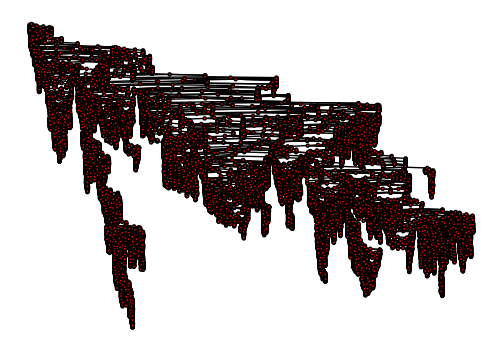
\includegraphics[width=7cm]{exempleIntro}<1->\\
		\begin{block}{Principe 1}<2->
		Les arêtes de l'arbre ne doivent pas s'intersecter.
		\end{block}
	\end{center}
\end{frame}

\begin{frame}
	\begin{center}	
		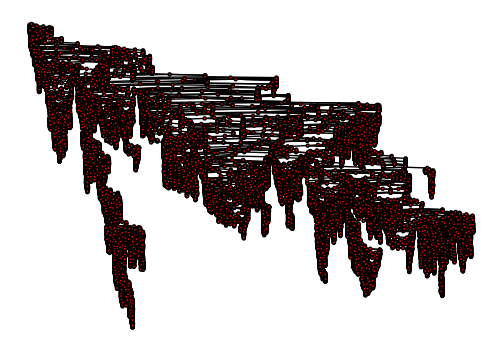
\includegraphics[width=7cm]{exempleIntro}<1->\\
		\begin{block}{Principe 2}<2->
		Les n\oe{}uds de même profondeur doivent être dessinés sur la même ligne horizontale.
		\end{block}
	\end{center}
\end{frame}

\begin{frame}
	\begin{center}	
		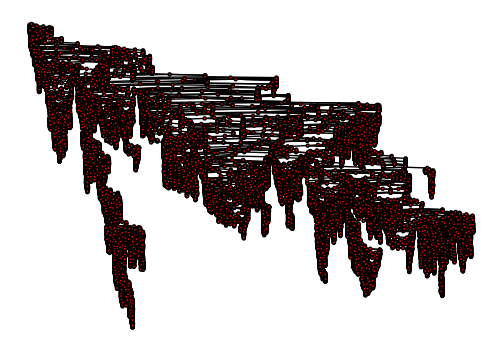
\includegraphics[width=7cm]{exempleIntro}<1->\\
		\begin{block}{Principe 3}<2->
		Les arbres doivent être dessinés de la manière la plus compacte possible.
		\end{block}
	\end{center}
\end{frame}

\begin{frame}
	\begin{center}	
		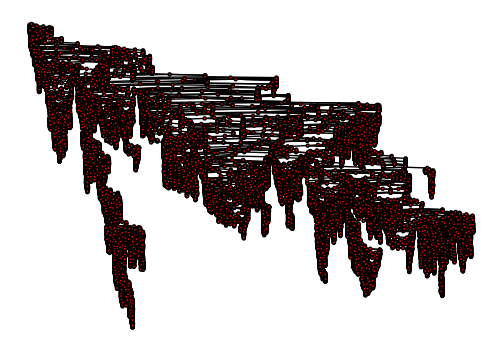
\includegraphics[width=7cm]{exempleIntro}<1->\\
		\begin{block}{Principe 4}<2->
		Un n\oe{}ud parent doit être centré par rapport à ses fils.
		\end{block}
	\end{center}
\end{frame}

\begin{frame}
	\begin{center}	
		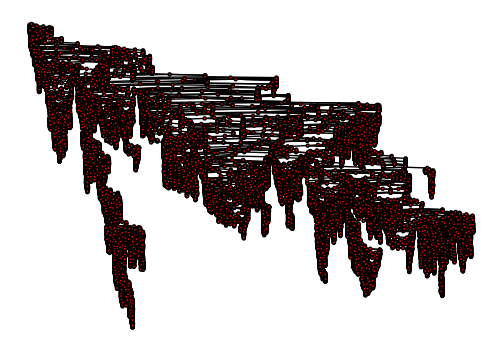
\includegraphics[width=7cm]{exempleIntro}<1->\\
		\begin{block}{Principe 5}<2->
		Un sous-arbre doit être dessiné de la même façon, peu importe où il est placé dans l'arbre.
		\end{block}
	\end{center}
\end{frame}

\begin{frame}
	\begin{center}	
		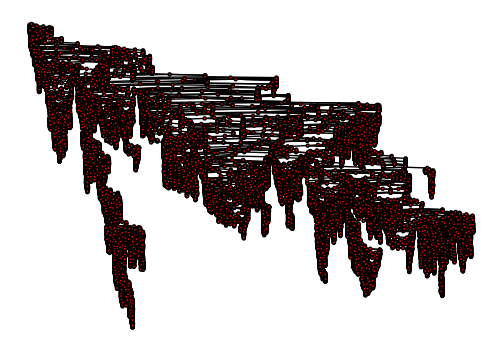
\includegraphics[width=7cm]{exempleIntro}<1->\\
		\begin{block}{Principe 6}<2->
		Les n\oe{}uds fils d'un n\oe{}ud père doivent être espacés de manière homogène.
		\end{block}
	\end{center}
\end{frame}

%\subsection{Algorithmes existants}
%
%\begin{frame}
%	\frametitle{Knuth}
%	\begin{center}
%	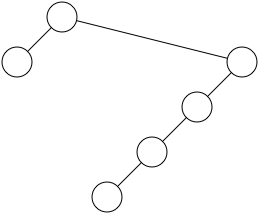
\includegraphics[height=3.5cm]{knuth}
%	\end{center}
%	Décrit une idée de "slot disponible"\\
%	Inconvénient :
%	\begin{itemize}
%		\item Ne respecte que les principes 1 et 2
%	\end{itemize}
%\end{frame}
%
%\begin{frame}
%	\frametitle{Algorithmes de Charles Wetherell et Alfred Shannon}
%	\begin{center}
%	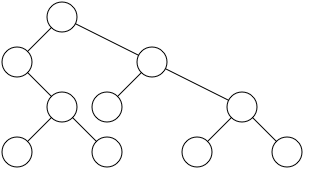
\includegraphics[height=3.5cm]{shannon}
%	\end{center}
%	Approche Bottom Up pour centrer le père sur ses fils\\
%	Introduction d'un tableau de slots\\
%	Inconvénient :
%	\begin{itemize}
%		\item Ne respecte pas les principes 4 et 5
%	\end{itemize}
%\end{frame}
%
%\begin{frame}
%	\frametitle{The Mods and the Rockers}
%	Traitement en deux passes\\
%	Avantage :
%	\begin{itemize}
%		\item Respecte tous les principes
%	\end{itemize}
%	Inconvénient
%	\begin{itemize}
%		\item Ne concerne que les arbres binaires
%	\end{itemize}
%\end{frame}

%\chapter{État des lieux}
%
%\paragraph{}Les articles que nous avons étudiés concernaient avant tout la visualisation des arbres binaires de grande taille sans prendre en compte l'ordre des fils. Il en ressort néanmoins plusieurs principes :
%\begin{enumerate}
%	\item Les arêtes de l'arbre ne doivent pas s'intersecter.
%	\item Les n\oe{}uds de même profondeur doivent être dessinés sur la même ligne horizontale.
%	\item Les arbres doivent être dessinés de la manière la plus compacte possible.
%	\item Un n\oe{}ud parent doit être centré par rapport à ses fils.
%	\item Un sous-arbre doit être dessiné de la même façon, peu importe où il est placé dans l'arbre.
%	\item Les n\oe{}uds fils d'un n\oe{}ud père doivent être espacés de manière homogène.
%\end{enumerate}
%
%\paragraph{}Un des enjeux soulevés par l'ensemble de ces principes est que les n\oe{}uds ne doivent pas se chevaucher, tout comme les arbres en eux-même.
%
%\paragraph{}Il existe plusieurs algorithmes permettant de dessiner des arbres de grande taille, mais tous ne respectent pas tous les principes décrits ci-dessus.
%
%\subparagraph{}Par exemple, l'algorithme le plus simple, l'algorithme de Knuth \cite{REF_Knuth}, ne respecte que les deux premiers principes. Cet algorithme décrit déjà une idée de "slot disponible". Mais ce sont Charles Wetherell et Alfred Shannon \cite{REF_Wetherell}, en 1979, qui introduiront l'utilisation d'un tableau qui associera à chaque profondeur le prochain slot disponible. Ils arrivent ainsi à respecter tous les principes, à l'exception des principes 4 et 5. Ils introduisent malgré tout également l'idée de parcourir l'arbre de bas en haut, plutôt que l'inverse, ceci afin de centrer facilement un père selon ses fils.
%
%\subparagraph{}Le principal problème est alors : Comment respecter tous ces principes et traiter le chevauchement d'arbres sans perdre en complexité ? C'est l'algorithme The Mods and the Rockers qui répondra à cette question. Au lieu de reparcourir les sous-arbres pour les décaler afin d'éviter tout chevauchement, on raisonne en deux passes de l'arbre. Lors de la première passe, on mémorise un \emph{modifier} qui indiquera le décallage qui devra être appliqué sur chaque sous-arbre lors de la deuxième passe.
%
%\subparagraph{}Il existe enfin des algorithmes dont le but est surtout d'optimiser les concepts et algorithmes existants. Citons le concept de contour d'arbre, qui permet de ne parcourir que ce contour et donc de ne pas rentrer au c\oe{}ur de l'arbre. Ceci est un gain conséquent puisque nous traitons ici des arbres de grande taille, et donc potentiellement très larges.
%
%\paragraph{}Nous allons donc voir à présent comment nous nous sommes inspirées de ces algorithmes afin de généraliser les concepts aux arbres n-aires, et en conservant l'ordre des fils. %Présentation des algos
\section{Étude de départ}

\subsection{TikZ}

\begin{frame}
	\frametitle{TikZ - Arbre de grande taille}
	Pas plus de 576 n\oe uds !
\end{frame}

\begin{frame}
	\frametitle{TikZ - Arbre de petite taille avec labels}
	image arbre avec labels
\end{frame}

\subsection{Asymptote}

\begin{frame}
	\frametitle{Asymptote - Arbre de grande taille}
	image arbre
\end{frame}

\begin{frame}
	\frametitle{Asymptote - Arbre de petite taille avec labels}
	image arbre avec labels
\end{frame}

\subsection{NetworkX + Matplotlib}

\begin{frame}
	\frametitle{NetworkX - Arbre de grande taille}
	image arbre
\end{frame}

\begin{frame}
	\frametitle{NetworkX - Arbre de petite taille avec labels}
	image arbre avec labels
\end{frame}


%\chapter{Étude préliminaire}
%
%\paragraph{}Le but de cette étude préliminaire est de trouver un outil adapté à la représentation d'arbres de grande taille. Étudions les performances de TikZ, Asymptote et NetworkX pour la génération d'un cas particulier d'arbres: les chaînes.
%
%	\section{TikZ}
%
%\paragraph{}TikZ est un package \LaTeX{} permettant la création de graphiques.
%
%\paragraph{}On va utiliser le code Python suivant pour générer du code TikZ décrivant un arbre linéaire d'une taille passée en paramètre.
%\lstinputlisting[language=Python]{testTikz.py}
%
%		\subsection{$500$ n\oe uds}
%
%\paragraph{}On utilise le code précédent pour générer un arbre linéaire de taille $500$. On insère le code obtenu dans un fichier \LaTeX{} pour voir le résultat. Le fichier \LaTeX{} compile et le résultat est aux figures \ref{arbre500TikZA} et \ref{arbre500TikZB}.
%
%		\subsection{$10000$ n\oe uds}
%		
%\paragraph{}On utilise maintenant le même code mais pour avoir un arbre de $10000$ n\oe uds. Le fichier \LaTeX{} ne compile plus. On obtient l'erreur \verb|dimension too large| à la ligne:
%\begin{lstlisting}
%\node (a576) at (0,576) {$576$};
%\end{lstlisting}
%
%\paragraph{} Si l'arbre est trop grand, essayons de réduire sa taille: on diminue l'échelle, on diminue la distance entre deux points et on supprime les labels. L'erreur persiste au même endroit. TikZ limite notre arbre à $575$ n\oe uds à la verticale. Peut-être la limite serait-elle différente si les n\oe uds était répartis autrement.
%
%	\section{Asymptote}
%
%\paragraph{}Asymptote est un langage de description de dessins vectoriels. Un package permet de le compiler dans un fichier \LaTeX{} mais le code asymptote peut aussi être autonome.
%
%\paragraph{}On va utiliser le code Python suivant pour générer du code Asymptote décrivant un arbre linéaire d'une taille passée en paramètre.
%\lstinputlisting[language=Python]{testAsymptote.py}
%
%		\subsection{$500$ n\oe uds}
%		
%\paragraph{}On commence doucement en générant un arbre de $500$ n\oe uds. On insère le code obtenu dans un fichier \LaTeX{} comme précédemment. Le fichier compile et le résultat obtenu est celui des figures \ref{arbre500AsyA} et \ref{arbre500AsyB}.
%
%		\subsection{$10000$ n\oe uds}
%\paragraph{}On recommence en mettant la barre à $10000$ n\oe uds. Le fichier compile sans problème et le résultat est celui des figures \ref{arbre10000AsyA} et \ref{arbre10000AsyB}.
%	
%	\section{NetworkX accompagné de Matplotlib}
%	
%\paragraph{}NetworkX est une bibliothèque Python pour l'étude des graphes, conçue pour fonctionner sur des grands graphes.
%
%\paragraph{}Matplotlib est aussi une bibliothèque Python mais qui permet quant à elle de générer une image 2D dans différents formats de sortie possible comme par exemple un png, un pdf ou un svg.
%
%\paragraph{}On va utiliser le code Python suivant pour générer du code NetworkX décrivant un arbre linéaire d'une taille passée en paramètre.
%\lstinputlisting[language=Python]{testNetworkx.py}
%
%		\subsection{$500$ n\oe uds}
%\paragraph{}De même que précédemment, on génère d'abord un arbre de $500$ n\oe uds. On choisi le format de sortie png. Le résultat est visible aux figures \ref{arbre500NkxA} et \ref{arbre500NkxB}.
%		
%		\subsection{$10000$ n\oe uds}
%\paragraph{}Passons maintenant à $10000$ n\oe uds. Le résultat est aux figures \ref{arbre10000NkxA} et \ref{arbre10000NkxB}.
%	
%	\section{Conclusion}
%	
%\paragraph{}TikZ permet une représentation claire d'un arbre avec ses labels. En effet, même avec $500$ n\oe uds, les labels sont lisibles si on zoome suffisamment. Cependant, une limite a rapidement été atteinte. TikZ serait préférable pour la représentation de petits arbres avec (ou sans!) labels.
%\paragraph{}Asymptote permet de représenter de grands arbres. Son point faible est la représentation des labels. Cependant, les labels sont compilés avec \LaTeX{} ce qui peut permettre d'avoir des labels un peu plus évolués qu'une chaîne de caractères, une fois la taille des labels maîtrisée.
%\paragraph{}NetworkX et Matplotlib permettent plusieurs formats de sortie différents. Cela pourrait être utile aux non-utilisateurs de \LaTeX{}. Cependant, l'affichage des labels n'est pas non plus très optimal.
%\paragraph{}Notons tout de même que cette étude préliminaire ne prend pas en compte le temps de calcul des coordonnées, ce qui est le c\oe ur de notre projet et qui est expliqué dans le chapitre suivant.
 %Présentation de l'étude préliminaire
\chapter{Choix d'implémentation}

\section{Fonctionnement général}

\paragraph{}L'utilisateur fourni un fichier et précise son type. Il peut aussi choisir d'afficher des labels sur les n\oe uds ainsi que le format de sortie souhaité. Par défaut, l'application génère un png sans labels. L'application fonctionne ensuite en trois étapes:
\begin{enumerate}
	\item Parsing du fichier d'entrée selon le type indiqué pour obtenir une représentation d'arbre selon notre structure interne.
	\item Calcul des coordonnées de chaque n\oe ud.
	\item Génération d'une image selon le type de sortie choisie.
\end{enumerate}

\begin{center}
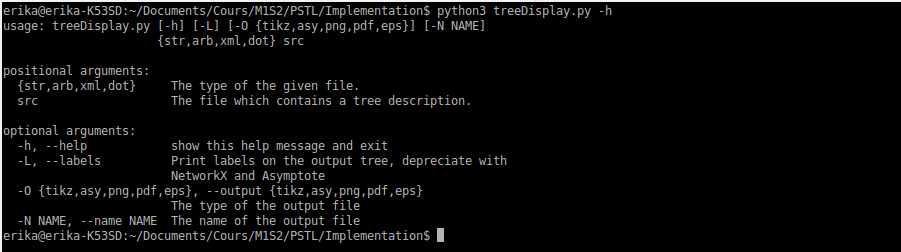
\includegraphics[width=\columnwidth]{usage}
\end{center}

\section{Plus en détails}

	\subsection{Structure d'arbre}
	
\lstinputlisting[language=Python, firstline=4, lastline=17]{../Implementation/tree.py}

	\subsection{Fonctionnement des algorithmes de parsing}

\paragraph{Mots bien parenthésés}Le parser de mots bien parenthésés (cf. \ref{dotParser}) respecte la grammaire suivante:
		
\begin{verbatim}
ARBRE : '(' ID NOEUDS ')'
NOEUDS : ARBRE NOEUDS | e
ID : [a-zA-Z1-9]* | e
\end{verbatim}
		
\paragraph{Dot}Le parser dot parse une sous-partie du langage dot, à savoir:

\begin{verbatim}
DOT : STRICT GRAPH ID '{' SEQINST '}'
STRICT : strict | e
GRAPH = diagraph | graph
SEQINST : INST SEQINST | e
INST : REF [label = "ID"] ';' | REF LINK REF
LINK : -- | ->
REF : [0-9]*
ID : [a-zA-Z1-9]* | e
\end{verbatim}
		
\paragraph{XML}Le parser XML utilise la librairie XML de Python. Il respecte la grammaire suivante:
		
\begin{verbatim}
XML : <?xml version="1.0"?><tree> NOEUDS <tree>
NOEUDS : NOEUD NOEUDS | e
NOEUD : <node type=TAG id=ID> NOEUDS </noeud> | <leaf type=TAG id=ID />
TAG : "Leaf" | "BinNode"
\end{verbatim}

	\subsection{Fonctionnement de l'algorithme de calcul de coordonnées}

\paragraph{}On décide que la distance minimale entre deux n\oe uds est de $1$ unité.

\paragraph{}L'ordonnée d'un n\oe ud est triviale: c'est sa profondeur.

\paragraph{}L'abcisse d'un n\oe ud est un peu plus complexe et demande donc plus de réflexion. Pour un n\oe ud donné, on commence par placer ses fils. On centre ensuite ce n\oe ud au milieu de ses fils en faisant la moyenne de l'absisse de ses deux fils extrémaux. Si un n\oe ud n'a pas de fils, on le place à $1$ de son frère gauche. D'un point de vue de l'architecture, on a donc besoin d'une structure qui, à profondeur \emph{p} mémorise la prochaine place disponible (ou au choix la dernière place utilisée.\\
Si un père a des fils, on le centre au milieu de ses fils. Par ce calcul, on peut se retrouver avec un n\oe ud qui est trop proche de son frère gauche [Mettre un exemple]. Pour cela, on compare la position calculée avec la première position disponible et on prend le max. Si la position calculée n'est pas celle retenue, le père n'est plus centré au milieu de ses fils. On mémorise donc le décalage effectué pour ce père pour ensuite l'appliquer à ses sous-arbre dans un second temps.
\begin{enumerate}
	\item Pour un n\oe ud donné, on commence par placer ses fils.
	\item On centre ensuite ce n\oe ud au milieu de ses fils.
	\item Si un n\oe ud collisionne avec son frère gauche, on le décale vers la droite et on mémorise ce décalage car il faudra ensuite décaler ses sous-arbres. On applique ce décalage dans une seconde passe pour des raisons de complexité. En effet, si on faisait chaque décalage lorsqu'il se présentait, le décalage serait quadratique alors que dans le cas choisi, on est linéaire.
\end{enumerate}

	\subsection{Fonctionnement de la génération du code}
	
\paragraph{TikZ}
		
\paragraph{Asymptote}
		
\paragraph{Autre}

\section{Complexité}

\paragraph{}On suppose que la taille des labels est bornée. On note $n$ le nombre de n\oe uds dans l'arbre. Dans ce cas:

\begin{enumerate}
	\item Le parsing d'un fichier est en $O(n)$.
	\item Le calcul des coordonnées est en $O(n)$ (on effectue $2$ passes sur l'arbre).
	\item La génération du fichier de sortie est en $O(n)$.
\end{enumerate}
On a donc une complexité générale en $O(n)$ où $n$ est le nombre de n\oe ud de l'arbre.

\paragraph{}Notons que nous avons supposé que la taille des labels était bornée. Or nous n'avons aucune prise sur la taille des labels du fichier qui nous est passé en entrée. Dans ce cas, même si on borne la taille des labels pour l'affichage, la complexité est dominée par le parsing du fichier d'entrée car on doit lire tous les caractères du fichier. %Présentation des choix effectués
\section{Étude de performances}

\begin{frame}
	\frametitle{Protocole}
	\begin{itemize}
		\item Une centaine d'arbres de taille de l'ordre de $10^{0}$ à $10^{5}$ générés aléatoirement
		\item Chaque instruction (parser, calcul des coordonnées, générateur) exécutée entre 5 et 10 fois
		\item Moyenne des temps d'exécution pour chaque instruction
	\end{itemize}
\end{frame}

\begin{frame}
	\frametitle{Bilan général}
	Meilleur cas (XML + Asymptote ou TikZ):
	\begin{itemize}
		\item Parser $\sim$ 40\% du temps d'exécution
		\item Calcul des coordonnées $\sim$ 30\% du temps d'exécution
		\item Génération de la sortie $\sim$ 30\% du temps d'exécution
	\end{itemize}
	Pire cas (DOT + NetworkX):
	\begin{itemize}
		\item Parser $\sim$ 10\% du temps d'exécution
		\item Calcul des coordonnées $\sim$ 1\% du temps d'exécution
		\item Génération de la sortie $\sim$ 89\% du temps d'exécution
	\end{itemize}
\end{frame}

\begin{frame}
	\frametitle{Calcul des coordonnées}
	\begin{center}
	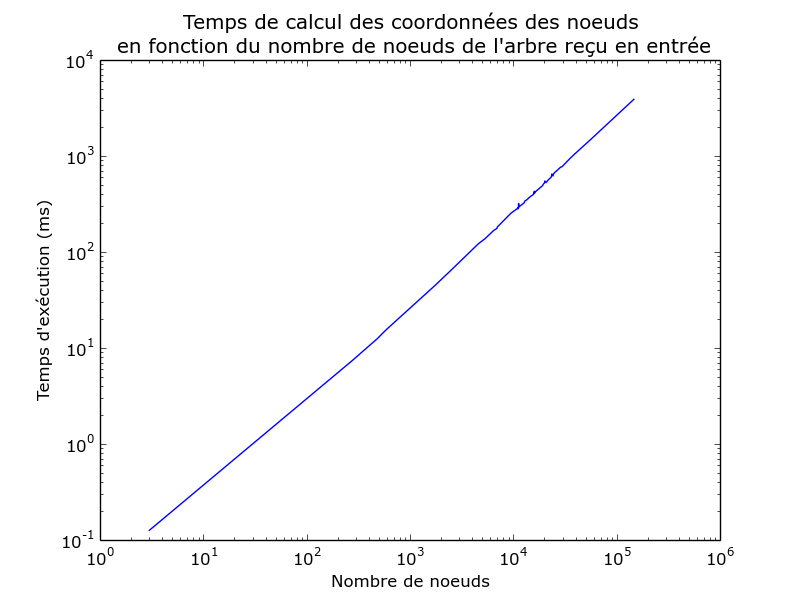
\includegraphics[height=7cm]{execTimeCoord}
	\end{center}
\end{frame}

\begin{frame}
	\frametitle{GraphViz vs TreeDisplay}
	\begin{center}
	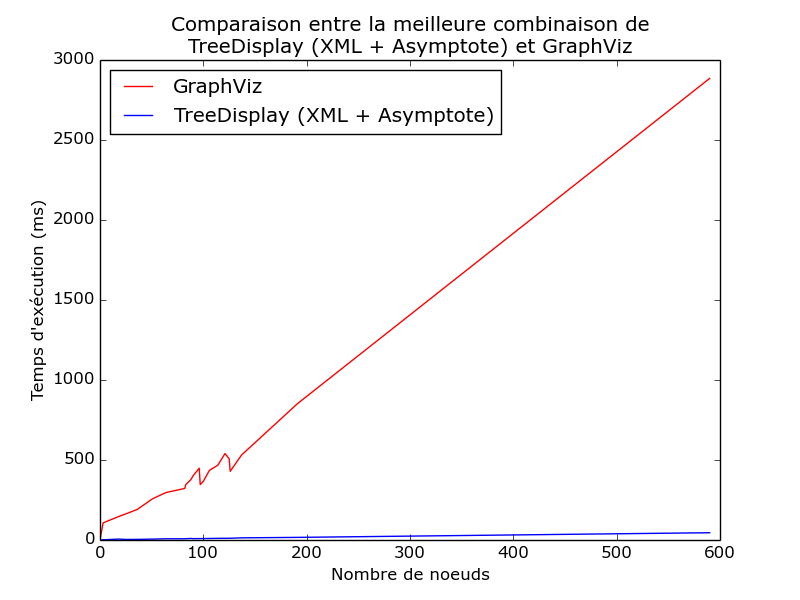
\includegraphics[height=7cm]{execTimeGV}
	\end{center}
\end{frame}



%\chapter{Étude de performances}
%
%\paragraph{} Avant toute chose, il est important de préciser que les tests effectués ci-dessous ont été réalisés sans aucun label. Comme expliqué précédemment, nous pouvons considérer que si la taille des labels est constante, la complexité des algorithme ne dépendra que du nombre de n\oe uds compris dans l'arbre. C'est donc l'hypothèse que nous faisons ici.
%
%	\section{Comparaison des temps d'exécution des différents parsers.}
%	
%\begin{center}
%
%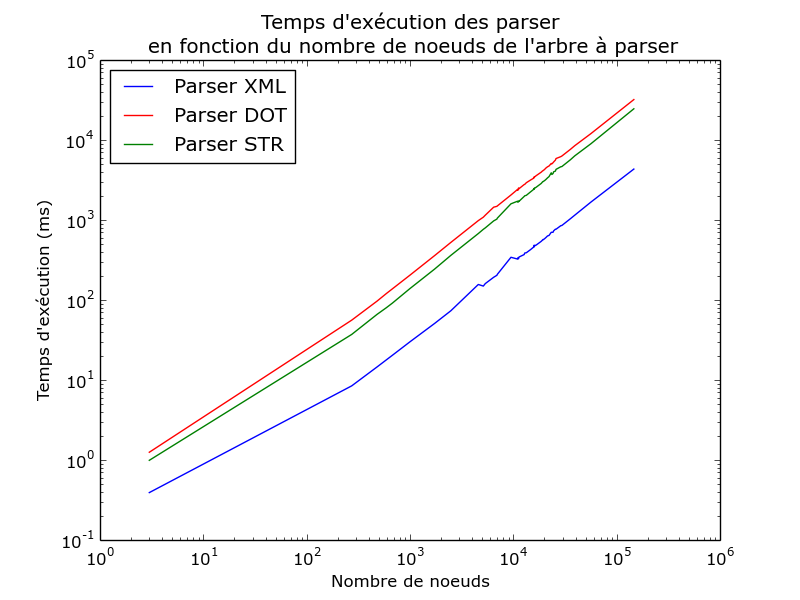
\includegraphics[width=\columnwidth]{execTimeParsers}
%
%\end{center}
%
%\paragraph{} Comme on avait pu le déduire précédemment, on peut observer que les parser ont une complexité linéaire. Ce qu'il ressort également de cette comparaison, c'est que le parser XML est le plus efficace des trois. Cela est certainement du au fait que nous utilisons un module interne à Python pour traiter le fichier d'entrée. En effet, les modules internes des langages sont généralement bien optimisés car pensés pour le langage concerné. De plus, en à peine une dizaine de secondes, nous pouvons parser un arbre contenant un million de n\oe uds.
%
%	\section{Évolution du temps de calcul des coordonées en fonction du nombre de n\oe uds de l'arbre.}
%	
%\begin{center}
%
%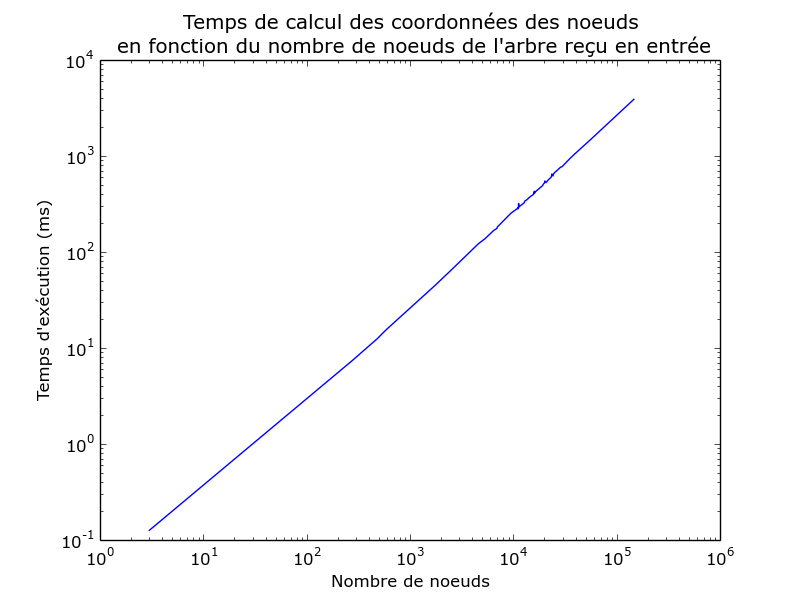
\includegraphics[width=\columnwidth]{execTimeCoord}
%
%\end{center}
%
%\paragraph{} Cette fois encore, le temps d'exécution de la méthode est d'une complexité linéaire. Nous pouvons également supposer, en observant l'évolution de la courbe, que pour un million de n\oe uds, nous n'aurions besoin que d'à peine une seconde pour effectuer le calcul de coordonnées, ce qui est un excellent résultat.
%
%	\section{Comparaison des temps d'exécution des différents générateurs.}
%
%\begin{center}
%
%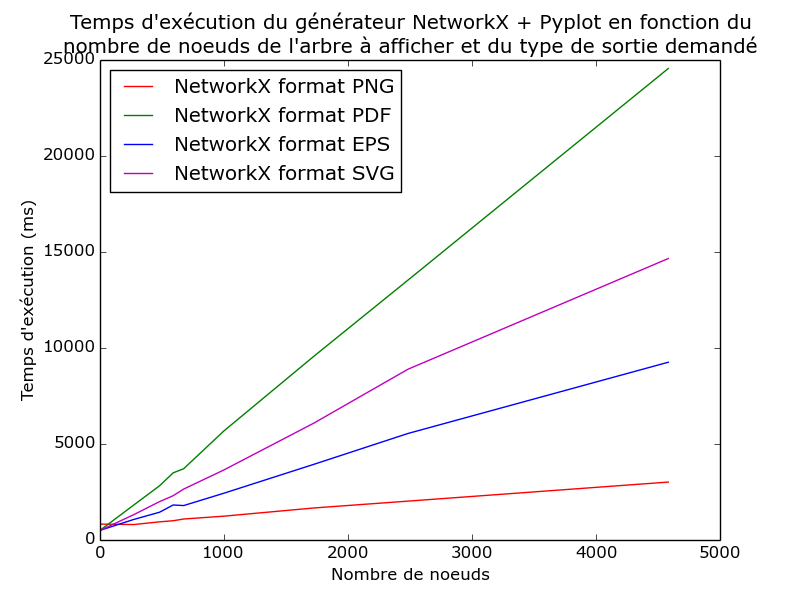
\includegraphics[width=\columnwidth]{execTimeNX}
%
%\end{center}
%
%\paragraph{} Nous comparons tout d'abord les différentes sorties gérées par NetworkX. Nous observons que nous sommes toujours en complexité linéaire, mais que le temps d'exécution est bien supérieur à ce qui peut être acceptable, avec plusieurs secondes pour seulement 5000 n\oe uds. Cependant, la complexité de ce générateur vient en grande partie du fait qu'il génère une image via MatplotLib. Ceci ralentit grandement l'exécution.
%	
%\begin{center}
%
%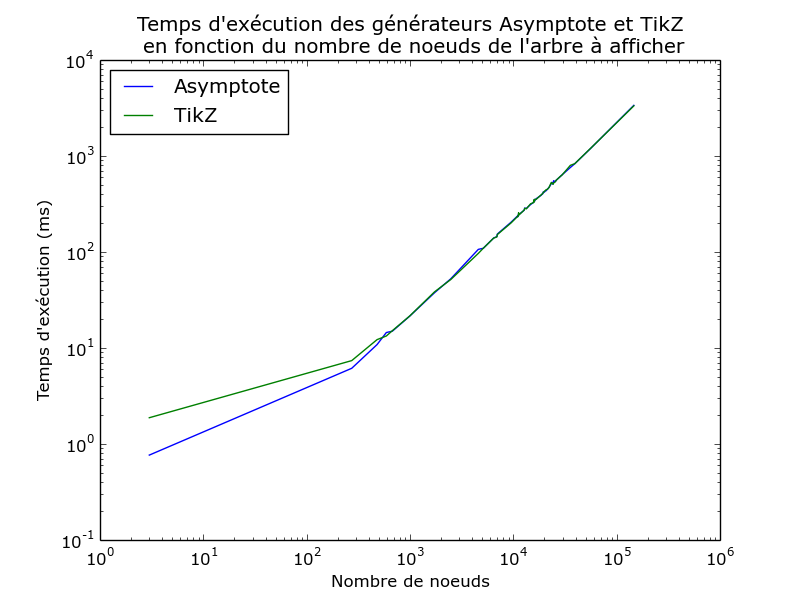
\includegraphics[width=\columnwidth]{execTimeGenerators}
%
%\end{center}
%
%\paragraph{} Contrairement à NetworkX, nous générons ici un fichier qui doit être recompilé. Ceci explique certainement en partie le fait que ce générateur soit plus efficace que le générateur NetworkX. Cependant, nous restons toujours en complexité linéaire.
%
%	\section{Comparaison des temps d'exécution entre GraphViz et la meilleur combinaison parser/générateur de TreeDisplay.}
%	
%\begin{center}
%
%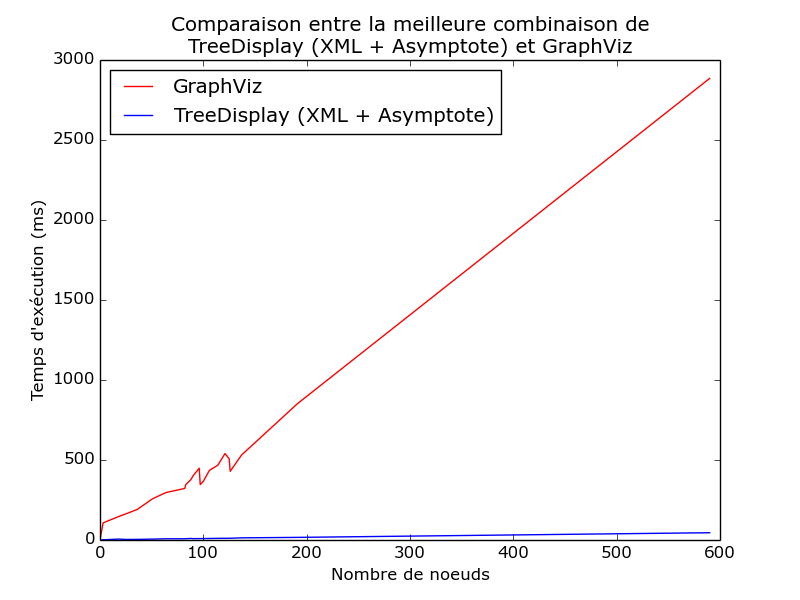
\includegraphics[width=\columnwidth]{execTimeGV}
%
%\end{center}
%
%\paragraph{} Nous comparons maintenant TreeDisplay dans sa meilleure combinaison possible de parser et de générateur de sortie, avec le visualiseur que nous avons cité en début de ce rapport : GraphViz. Il en ressort que TreeDisplay est bien plus puissant que GraphViz. Cependant, GraphViz gère des graphes de manière générale et fournit une image en sortie, et nous avons généré un fichier .tex à compiler. Ceci peut expliquer en partie la différence de performance.
\chapter{Comparaison des affichages}

	\section{Avec labels}
	
\paragraph{}Nous allons à présent comparer le rendu visuel de nos différents générateurs ainsi que de GraphViz qui est de nos jours l'outil le plus utilisé.

\paragraph{TikZ} Nous commençons ce comparatif avec TikZ, qui offre un affichage des labels optimisés.\\

\begin{center}
\resizebox {!}{7cm} {
\begin{tikzpicture}[scale=0.8, every node/.style={scale=0.8}, node distance=1pt]
\node (a3027826572) at (3.500000, -0.000000) {1};
\node (a3027828524) at (3.500000, -1.000000) {2};
\node (a3027828204) at (3.500000, -2.000000) {3};
\node (a3027827948) at (2.000000, -3.000000) {4};
\node (a3027826636) at (1.500000, -4.000000) {7};
\node (a3027826988) at (1.000000, -5.000000) {12};
\node (a3027826604) at (0.500000, -6.000000) {16};
\node (a3027830572) at (0.500000, -7.000000) {18};
\node (a3027830092) at (0.500000, -8.000000) {19};
\node (a3027832332) at (0.000000, -9.000000) {20};
\draw (a3027830092) -- (a3027832332);
\node (a3027832396) at (1.000000, -9.000000) {21};
\draw (a3027830092) -- (a3027832396);
\draw (a3027830572) -- (a3027830092);
\draw (a3027826604) -- (a3027830572);
\draw (a3027826988) -- (a3027826604);
\node (a3027832556) at (1.500000, -6.000000) {17};
\draw (a3027826988) -- (a3027832556);
\draw (a3027826636) -- (a3027826988);
\node (a3027832684) at (2.000000, -5.000000) {13};
\draw (a3027826636) -- (a3027832684);
\draw (a3027827948) -- (a3027826636);
\node (a3027832812) at (2.500000, -4.000000) {8};
\draw (a3027827948) -- (a3027832812);
\draw (a3027828204) -- (a3027827948);
\node (a3027849356) at (3.500000, -3.000000) {5};
\node (a3027849388) at (3.500000, -4.000000) {9};
\node (a3027849420) at (3.000000, -5.000000) {14};
\draw (a3027849388) -- (a3027849420);
\node (a3027849516) at (4.000000, -5.000000) {15};
\draw (a3027849388) -- (a3027849516);
\draw (a3027849356) -- (a3027849388);
\draw (a3027828204) -- (a3027849356);
\node (a3027849676) at (5.000000, -3.000000) {6};
\node (a3027849708) at (4.500000, -4.000000) {10};
\draw (a3027849676) -- (a3027849708);
\node (a3027849804) at (5.500000, -4.000000) {11};
\draw (a3027849676) -- (a3027849804);
\draw (a3027828204) -- (a3027849676);
\draw (a3027828524) -- (a3027828204);
\draw (a3027826572) -- (a3027828524);

\end{tikzpicture}}
\end{center}

\paragraph{Asymptote} Continuons avec le deuxième format \LaTeX de notre application qu'est Asymptote.\\

\begin{center}
\begin{asy}
size(20cm, 20cm);
label("1", (3.500000, -0.000000), E);
label("2", (3.500000, -1.000000), E);
label("3", (3.500000, -2.000000), E);
label("4", (2.000000, -3.000000), E);
label("7", (1.500000, -4.000000), E);
label("12", (1.000000, -5.000000), E);
label("16", (0.500000, -6.000000), E);
label("18", (0.500000, -7.000000), E);
label("19", (0.500000, -8.000000), E);
label("20", (0.000000, -9.000000), E);
draw((0.500000, -8.000000) -- (0.000000, -9.000000));
label("21", (1.000000, -9.000000), E);
draw((0.500000, -8.000000) -- (1.000000, -9.000000));
draw((0.500000, -7.000000) -- (0.500000, -8.000000));
draw((0.500000, -6.000000) -- (0.500000, -7.000000));
draw((1.000000, -5.000000) -- (0.500000, -6.000000));
label("17", (1.500000, -6.000000), E);
draw((1.000000, -5.000000) -- (1.500000, -6.000000));
draw((1.500000, -4.000000) -- (1.000000, -5.000000));
label("13", (2.000000, -5.000000), E);
draw((1.500000, -4.000000) -- (2.000000, -5.000000));
draw((2.000000, -3.000000) -- (1.500000, -4.000000));
label("8", (2.500000, -4.000000), E);
draw((2.000000, -3.000000) -- (2.500000, -4.000000));
draw((3.500000, -2.000000) -- (2.000000, -3.000000));
label("5", (3.500000, -3.000000), E);
label("9", (3.500000, -4.000000), E);
label("14", (3.000000, -5.000000), E);
draw((3.500000, -4.000000) -- (3.000000, -5.000000));
label("15", (4.000000, -5.000000), E);
draw((3.500000, -4.000000) -- (4.000000, -5.000000));
draw((3.500000, -3.000000) -- (3.500000, -4.000000));
draw((3.500000, -2.000000) -- (3.500000, -3.000000));
label("6", (5.000000, -3.000000), E);
label("10", (4.500000, -4.000000), E);
draw((5.000000, -3.000000) -- (4.500000, -4.000000));
label("11", (5.500000, -4.000000), E);
draw((5.000000, -3.000000) -- (5.500000, -4.000000));
draw((3.500000, -2.000000) -- (5.000000, -3.000000));
draw((3.500000, -1.000000) -- (3.500000, -2.000000));
draw((3.500000, -0.000000) -- (3.500000, -1.000000));
\end{asy}

\end{center}

\subparagraph{} L'avantage d'Asymptote réside dans le fait que les labels sont compilés avec \LaTeX. Voici donc un exemple supplémentaire pour montrer les possibilités offerte avec Asymptote.\\

\begin{center}
\begin{asy}
size(20cm, 20cm);
label("1", (3.500000, -0.000000), E);
label("2", (3.500000, -1.000000), E);
label("3", (3.500000, -2.000000), E);
label("4", (2.000000, -3.000000), E);
label("7", (1.500000, -4.000000), E);
label("12", (1.000000, -5.000000), E);
label("16", (0.500000, -6.000000), E);
label("18", (0.500000, -7.000000), E);
label("19", (0.500000, -8.000000), E);
label("20", (0.000000, -9.000000), E);
draw((0.500000, -8.000000) -- (0.000000, -9.000000));
label("21", (1.000000, -9.000000), E);
draw((0.500000, -8.000000) -- (1.000000, -9.000000));
draw((0.500000, -7.000000) -- (0.500000, -8.000000));
draw((0.500000, -6.000000) -- (0.500000, -7.000000));
draw((1.000000, -5.000000) -- (0.500000, -6.000000));
label("17", (1.500000, -6.000000), E);
draw((1.000000, -5.000000) -- (1.500000, -6.000000));
draw((1.500000, -4.000000) -- (1.000000, -5.000000));
label("13", (2.000000, -5.000000), E);
draw((1.500000, -4.000000) -- (2.000000, -5.000000));
draw((2.000000, -3.000000) -- (1.500000, -4.000000));
label("8", (2.500000, -4.000000), E);
draw((2.000000, -3.000000) -- (2.500000, -4.000000));
draw((3.500000, -2.000000) -- (2.000000, -3.000000));
label("5", (3.500000, -3.000000), E);
label("9", (3.500000, -4.000000), E);
label("14", (3.000000, -5.000000), E);
draw((3.500000, -4.000000) -- (3.000000, -5.000000));
label("15", (4.000000, -5.000000), E);
draw((3.500000, -4.000000) -- (4.000000, -5.000000));
draw((3.500000, -3.000000) -- (3.500000, -4.000000));
draw((3.500000, -2.000000) -- (3.500000, -3.000000));
label("6", (5.000000, -3.000000), E);
label("10", (4.500000, -4.000000), E);
draw((5.000000, -3.000000) -- (4.500000, -4.000000));
label("11", (5.500000, -4.000000), E);
draw((5.000000, -3.000000) -- (5.500000, -4.000000));
draw((3.500000, -2.000000) -- (5.000000, -3.000000));
draw((3.500000, -1.000000) -- (3.500000, -2.000000));
draw((3.500000, -0.000000) -- (3.500000, -1.000000));
\end{asy}

\end{center}

\paragraph{NetworkX} Le dernier rendu, que l'on peut obtenir sous la forme de plusieurs format de fichiers est le suivant:\\

\begin{center}
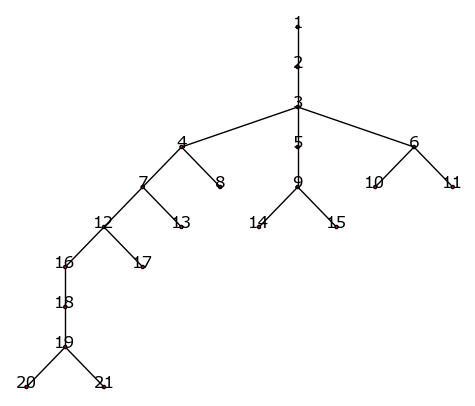
\includegraphics[height=7cm]{renduNXLabels}
\end{center}
	
\paragraph{GraphViz} Voici pour finir ce comparatif le rendu de GraphViz pour le même arbre.\\

\begin{center}
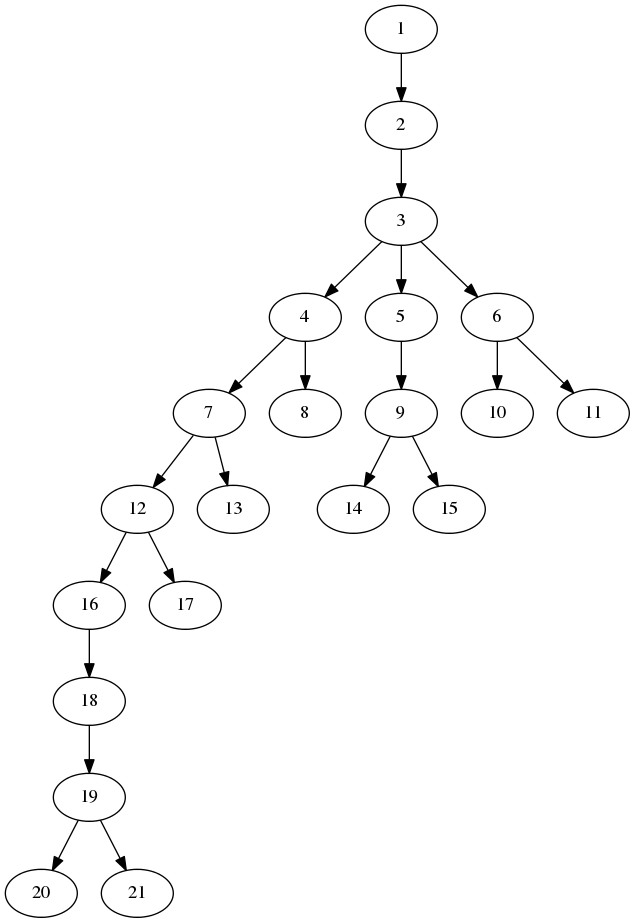
\includegraphics[height=7cm]{renduGVLabels}
\end{center}
	
	\section{Sans labels}

\paragraph{TikZ}

\begin{center}
\resizebox {!}{0.50\columnwidth} {
\begin{tikzpicture}[scale=0.8, every node/.style={scale=0.8}, node distance=1pt]
\draw (0.500000, -4.000000) -- (0.000000, -5.000000);
\draw (1.000000, -5.000000) -- (1.000000, -6.000000);
\draw (0.500000, -4.000000) -- (1.000000, -5.000000);
\draw (0.500000, -3.000000) -- (0.500000, -4.000000);
\draw (7.967918, -2.000000) -- (0.500000, -3.000000);
\draw (7.967918, -2.000000) -- (1.500000, -3.000000);
\draw (2.000000, -7.000000) -- (1.000000, -8.000000);
\draw (2.000000, -7.000000) -- (2.000000, -8.000000);
\draw (2.000000, -7.000000) -- (3.000000, -8.000000);
\draw (2.500000, -6.000000) -- (2.000000, -7.000000);
\draw (2.500000, -6.000000) -- (3.000000, -7.000000);
\draw (3.250000, -5.000000) -- (2.500000, -6.000000);
\draw (4.000000, -6.000000) -- (4.000000, -7.000000);
\draw (3.250000, -5.000000) -- (4.000000, -6.000000);
\draw (14.435836, -4.000000) -- (3.250000, -5.000000);
\draw (25.621671, -5.000000) -- (5.000000, -6.000000);
\draw (6.000000, -6.000000) -- (6.000000, -7.000000);
\draw (25.621671, -5.000000) -- (6.000000, -6.000000);
\draw (13.210886, -7.000000) -- (5.000000, -8.000000);
\draw (6.000000, -9.000000) -- (6.000000, -10.000000);
\draw (6.000000, -8.000000) -- (6.000000, -9.000000);
\draw (13.210886, -7.000000) -- (6.000000, -8.000000);
\draw (17.171772, -11.000000) -- (6.000000, -12.000000);
\draw (17.171772, -11.000000) -- (7.000000, -12.000000);
\draw (7.000000, -14.000000) -- (6.000000, -15.000000);
\draw (7.000000, -14.000000) -- (7.000000, -15.000000);
\draw (7.000000, -14.000000) -- (8.000000, -15.000000);
\draw (15.748047, -13.000000) -- (7.000000, -14.000000);
\draw (6.000000, -17.000000) -- (6.000000, -18.000000);
\draw (8.576172, -16.000000) -- (6.000000, -17.000000);
\draw (6.000000, -21.000000) -- (6.000000, -22.000000);
\draw (6.000000, -20.000000) -- (6.000000, -21.000000);
\draw (6.000000, -19.000000) -- (6.000000, -20.000000);
\draw (11.152344, -18.000000) -- (6.000000, -19.000000);
\draw (6.000000, -23.000000) -- (6.000000, -24.000000);
\draw (8.875000, -22.000000) -- (6.000000, -23.000000);
\draw (6.750000, -25.000000) -- (6.000000, -26.000000);
\draw (7.500000, -26.000000) -- (6.000000, -27.000000);
\draw (7.500000, -26.000000) -- (7.000000, -27.000000);
\draw (7.500000, -26.000000) -- (8.000000, -27.000000);
\draw (7.500000, -26.000000) -- (9.000000, -27.000000);
\draw (6.750000, -25.000000) -- (7.500000, -26.000000);
\draw (8.125000, -24.000000) -- (6.750000, -25.000000);
\draw (8.500000, -25.000000) -- (8.500000, -26.000000);
\draw (8.125000, -24.000000) -- (8.500000, -25.000000);
\draw (8.125000, -24.000000) -- (9.500000, -25.000000);
\draw (8.125000, -23.000000) -- (8.125000, -24.000000);
\draw (8.875000, -22.000000) -- (8.125000, -23.000000);
\draw (8.875000, -22.000000) -- (9.125000, -23.000000);
\draw (10.000000, -26.000000) -- (10.000000, -27.000000);
\draw (11.000000, -25.000000) -- (10.000000, -26.000000);
\draw (11.000000, -26.000000) -- (11.000000, -27.000000);
\draw (11.000000, -25.000000) -- (11.000000, -26.000000);
\draw (11.000000, -25.000000) -- (12.000000, -26.000000);
\draw (11.000000, -24.000000) -- (11.000000, -25.000000);
\draw (11.750000, -23.000000) -- (11.000000, -24.000000);
\draw (12.500000, -24.000000) -- (12.000000, -25.000000);
\draw (12.500000, -24.000000) -- (13.000000, -25.000000);
\draw (11.750000, -23.000000) -- (12.500000, -24.000000);
\draw (8.875000, -22.000000) -- (11.750000, -23.000000);
\draw (8.875000, -21.000000) -- (8.875000, -22.000000);
\draw (8.875000, -20.000000) -- (8.875000, -21.000000);
\draw (16.304688, -19.000000) -- (8.875000, -20.000000);
\draw (10.875000, -20.000000) -- (9.875000, -21.000000);
\draw (10.875000, -20.000000) -- (10.875000, -21.000000);
\draw (11.875000, -21.000000) -- (11.875000, -22.000000);
\draw (10.875000, -20.000000) -- (11.875000, -21.000000);
\draw (16.304688, -19.000000) -- (10.875000, -20.000000);
\draw (13.375000, -20.000000) -- (12.875000, -21.000000);
\draw (13.875000, -21.000000) -- (13.875000, -22.000000);
\draw (13.375000, -20.000000) -- (13.875000, -21.000000);
\draw (16.304688, -19.000000) -- (13.375000, -20.000000);
\draw (19.781250, -21.000000) -- (14.875000, -22.000000);
\draw (19.781250, -21.000000) -- (15.875000, -22.000000);
\draw (16.875000, -22.000000) -- (16.875000, -23.000000);
\draw (19.781250, -21.000000) -- (16.875000, -22.000000);
\draw (19.875000, -23.000000) -- (17.625000, -24.000000);
\draw (16.875000, -28.000000) -- (16.875000, -29.000000);
\draw (16.875000, -27.000000) -- (16.875000, -28.000000);
\draw (18.125000, -26.000000) -- (16.875000, -27.000000);
\draw (17.875000, -27.000000) -- (17.875000, -28.000000);
\draw (18.125000, -26.000000) -- (17.875000, -27.000000);
\draw (19.375000, -27.000000) -- (18.875000, -28.000000);
\draw (19.375000, -27.000000) -- (19.875000, -28.000000);
\draw (18.125000, -26.000000) -- (19.375000, -27.000000);
\draw (18.125000, -25.000000) -- (18.125000, -26.000000);
\draw (22.125000, -24.000000) -- (18.125000, -25.000000);
\draw (20.875000, -28.000000) -- (20.375000, -29.000000);
\draw (21.375000, -29.000000) -- (21.375000, -30.000000);
\draw (20.875000, -28.000000) -- (21.375000, -29.000000);
\draw (22.125000, -27.000000) -- (20.875000, -28.000000);
\draw (22.375000, -31.000000) -- (22.375000, -32.000000);
\draw (22.375000, -30.000000) -- (22.375000, -31.000000);
\draw (22.375000, -29.000000) -- (22.375000, -30.000000);
\draw (23.375000, -28.000000) -- (22.375000, -29.000000);
\draw (23.375000, -28.000000) -- (23.375000, -29.000000);
\draw (23.375000, -28.000000) -- (24.375000, -29.000000);
\draw (22.125000, -27.000000) -- (23.375000, -28.000000);
\draw (22.125000, -26.000000) -- (22.125000, -27.000000);
\draw (23.125000, -25.000000) -- (22.125000, -26.000000);
\draw (23.125000, -25.000000) -- (23.125000, -26.000000);
\draw (23.125000, -25.000000) -- (24.125000, -26.000000);
\draw (22.125000, -24.000000) -- (23.125000, -25.000000);
\draw (25.125000, -25.000000) -- (25.125000, -26.000000);
\draw (22.125000, -24.000000) -- (25.125000, -25.000000);
\draw (25.625000, -27.000000) -- (24.625000, -28.000000);
\draw (25.625000, -27.000000) -- (25.625000, -28.000000);
\draw (25.625000, -27.000000) -- (26.625000, -28.000000);
\draw (26.125000, -26.000000) -- (25.625000, -27.000000);
\draw (26.125000, -26.000000) -- (26.625000, -27.000000);
\draw (26.125000, -25.000000) -- (26.125000, -26.000000);
\draw (22.125000, -24.000000) -- (26.125000, -25.000000);
\draw (19.875000, -23.000000) -- (22.125000, -24.000000);
\draw (24.687500, -22.000000) -- (19.875000, -23.000000);
\draw (29.500000, -23.000000) -- (23.125000, -24.000000);
\draw (29.125000, -27.000000) -- (27.625000, -28.000000);
\draw (27.875000, -36.000000) -- (27.875000, -37.000000);
\draw (27.875000, -35.000000) -- (27.875000, -36.000000);
\draw (27.875000, -34.000000) -- (27.875000, -35.000000);
\draw (27.875000, -33.000000) -- (27.875000, -34.000000);
\draw (27.875000, -32.000000) -- (27.875000, -33.000000);
\draw (28.625000, -31.000000) -- (27.875000, -32.000000);
\draw (28.875000, -33.000000) -- (28.875000, -34.000000);
\draw (29.375000, -32.000000) -- (28.875000, -33.000000);
\draw (29.875000, -34.000000) -- (29.875000, -35.000000);
\draw (29.875000, -33.000000) -- (29.875000, -34.000000);
\draw (29.375000, -32.000000) -- (29.875000, -33.000000);
\draw (28.625000, -31.000000) -- (29.375000, -32.000000);
\draw (28.625000, -30.000000) -- (28.625000, -31.000000);
\draw (28.625000, -29.000000) -- (28.625000, -30.000000);
\draw (28.625000, -28.000000) -- (28.625000, -29.000000);
\draw (29.125000, -27.000000) -- (28.625000, -28.000000);
\draw (29.125000, -27.000000) -- (29.625000, -28.000000);
\draw (29.125000, -27.000000) -- (30.625000, -28.000000);
\draw (29.125000, -26.000000) -- (29.125000, -27.000000);
\draw (30.125000, -25.000000) -- (29.125000, -26.000000);
\draw (30.125000, -25.000000) -- (30.125000, -26.000000);
\draw (30.125000, -25.000000) -- (31.125000, -26.000000);
\draw (31.375000, -24.000000) -- (30.125000, -25.000000);
\draw (32.625000, -25.000000) -- (32.125000, -26.000000);
\draw (32.625000, -25.000000) -- (33.125000, -26.000000);
\draw (31.375000, -24.000000) -- (32.625000, -25.000000);
\draw (29.500000, -23.000000) -- (31.375000, -24.000000);
\draw (35.875000, -24.000000) -- (33.625000, -25.000000);
\draw (34.125000, -27.000000) -- (34.125000, -28.000000);
\draw (34.125000, -26.000000) -- (34.125000, -27.000000);
\draw (35.125000, -25.000000) -- (34.125000, -26.000000);
\draw (35.125000, -25.000000) -- (35.125000, -26.000000);
\draw (34.625000, -31.000000) -- (34.625000, -32.000000);
\draw (34.625000, -30.000000) -- (34.625000, -31.000000);
\draw (35.125000, -29.000000) -- (34.625000, -30.000000);
\draw (35.125000, -29.000000) -- (35.625000, -30.000000);
\draw (35.125000, -28.000000) -- (35.125000, -29.000000);
\draw (35.125000, -27.000000) -- (35.125000, -28.000000);
\draw (36.125000, -26.000000) -- (35.125000, -27.000000);
\draw (36.125000, -26.000000) -- (36.125000, -27.000000);
\draw (37.125000, -27.000000) -- (36.125000, -28.000000);
\draw (37.125000, -28.000000) -- (37.125000, -29.000000);
\draw (37.125000, -27.000000) -- (37.125000, -28.000000);
\draw (37.125000, -27.000000) -- (38.125000, -28.000000);
\draw (36.125000, -26.000000) -- (37.125000, -27.000000);
\draw (35.125000, -25.000000) -- (36.125000, -26.000000);
\draw (35.875000, -24.000000) -- (35.125000, -25.000000);
\draw (35.875000, -24.000000) -- (36.125000, -25.000000);
\draw (35.875000, -24.000000) -- (37.125000, -25.000000);
\draw (35.875000, -24.000000) -- (38.125000, -25.000000);
\draw (29.500000, -23.000000) -- (35.875000, -24.000000);
\draw (24.687500, -22.000000) -- (29.500000, -23.000000);
\draw (19.781250, -21.000000) -- (24.687500, -22.000000);
\draw (22.734375, -20.000000) -- (19.781250, -21.000000);
\draw (22.734375, -20.000000) -- (20.781250, -21.000000);
\draw (25.687500, -21.000000) -- (25.687500, -22.000000);
\draw (22.734375, -20.000000) -- (25.687500, -21.000000);
\draw (16.304688, -19.000000) -- (22.734375, -20.000000);
\draw (16.304688, -19.000000) -- (23.734375, -20.000000);
\draw (11.152344, -18.000000) -- (16.304688, -19.000000);
\draw (11.152344, -17.000000) -- (11.152344, -18.000000);
\draw (8.576172, -16.000000) -- (11.152344, -17.000000);
\draw (13.440430, -15.000000) -- (8.576172, -16.000000);
\draw (12.652344, -16.000000) -- (12.152344, -17.000000);
\draw (12.652344, -16.000000) -- (13.152344, -17.000000);
\draw (13.440430, -15.000000) -- (12.652344, -16.000000);
\draw (13.440430, -15.000000) -- (13.652344, -16.000000);
\draw (13.440430, -15.000000) -- (14.652344, -16.000000);
\draw (17.304688, -18.000000) -- (17.304688, -19.000000);
\draw (18.304688, -17.000000) -- (17.304688, -18.000000);
\draw (18.304688, -17.000000) -- (18.304688, -18.000000);
\draw (18.304688, -17.000000) -- (19.304688, -18.000000);
\draw (18.304688, -16.000000) -- (18.304688, -17.000000);
\draw (13.440430, -15.000000) -- (18.304688, -16.000000);
\draw (13.440430, -14.000000) -- (13.440430, -15.000000);
\draw (15.748047, -13.000000) -- (13.440430, -14.000000);
\draw (24.496094, -17.000000) -- (20.304688, -18.000000);
\draw (26.687500, -21.000000) -- (26.687500, -22.000000);
\draw (27.187500, -20.000000) -- (26.687500, -21.000000);
\draw (27.187500, -20.000000) -- (27.687500, -21.000000);
\draw (27.187500, -19.000000) -- (27.187500, -20.000000);
\draw (28.687500, -18.000000) -- (27.187500, -19.000000);
\draw (28.687500, -18.000000) -- (28.187500, -19.000000);
\draw (28.687500, -18.000000) -- (29.187500, -19.000000);
\draw (30.187500, -19.000000) -- (29.687500, -20.000000);
\draw (30.187500, -19.000000) -- (30.687500, -20.000000);
\draw (28.687500, -18.000000) -- (30.187500, -19.000000);
\draw (24.496094, -17.000000) -- (28.687500, -18.000000);
\draw (24.496094, -16.000000) -- (24.496094, -17.000000);
\draw (24.496094, -15.000000) -- (24.496094, -16.000000);
\draw (24.496094, -14.000000) -- (24.496094, -15.000000);
\draw (15.748047, -13.000000) -- (24.496094, -14.000000);
\draw (28.343544, -12.000000) -- (15.748047, -13.000000);
\draw (25.496094, -15.000000) -- (25.496094, -16.000000);
\draw (25.496094, -14.000000) -- (25.496094, -15.000000);
\draw (26.496094, -13.000000) -- (25.496094, -14.000000);
\draw (26.496094, -13.000000) -- (26.496094, -14.000000);
\draw (27.496094, -14.000000) -- (27.496094, -15.000000);
\draw (26.496094, -13.000000) -- (27.496094, -14.000000);
\draw (28.343544, -12.000000) -- (26.496094, -13.000000);
\draw (27.496094, -16.000000) -- (27.496094, -17.000000);
\draw (31.591797, -15.000000) -- (27.496094, -16.000000);
\draw (31.591797, -15.000000) -- (28.496094, -16.000000);
\draw (32.687500, -17.000000) -- (31.687500, -18.000000);
\draw (32.687500, -17.000000) -- (32.687500, -18.000000);
\draw (32.687500, -17.000000) -- (33.687500, -18.000000);
\draw (33.187500, -16.000000) -- (32.687500, -17.000000);
\draw (33.187500, -16.000000) -- (33.687500, -17.000000);
\draw (31.591797, -15.000000) -- (33.187500, -16.000000);
\draw (35.687500, -16.000000) -- (34.687500, -17.000000);
\draw (35.687500, -17.000000) -- (35.687500, -18.000000);
\draw (35.687500, -16.000000) -- (35.687500, -17.000000);
\draw (35.687500, -16.000000) -- (36.687500, -17.000000);
\draw (31.591797, -15.000000) -- (35.687500, -16.000000);
\draw (40.439041, -14.000000) -- (31.591797, -15.000000);
\draw (37.687500, -16.000000) -- (37.687500, -17.000000);
\draw (42.986893, -15.000000) -- (37.687500, -16.000000);
\draw (39.187500, -16.000000) -- (38.687500, -17.000000);
\draw (39.187500, -16.000000) -- (39.687500, -17.000000);
\draw (42.986893, -15.000000) -- (39.187500, -16.000000);
\draw (47.786285, -17.000000) -- (36.687500, -18.000000);
\draw (36.687500, -19.000000) -- (36.687500, -20.000000);
\draw (37.687500, -18.000000) -- (36.687500, -19.000000);
\draw (37.687500, -20.000000) -- (37.687500, -21.000000);
\draw (38.687500, -19.000000) -- (37.687500, -20.000000);
\draw (38.687500, -19.000000) -- (38.687500, -20.000000);
\draw (39.687500, -20.000000) -- (39.687500, -21.000000);
\draw (38.687500, -19.000000) -- (39.687500, -20.000000);
\draw (37.687500, -18.000000) -- (38.687500, -19.000000);
\draw (47.786285, -17.000000) -- (37.687500, -18.000000);
\draw (47.786285, -18.000000) -- (39.687500, -19.000000);
\draw (47.786285, -18.000000) -- (40.687500, -19.000000);
\draw (55.885071, -19.000000) -- (40.687500, -20.000000);
\draw (40.687500, -21.000000) -- (40.187500, -22.000000);
\draw (40.687500, -21.000000) -- (41.187500, -22.000000);
\draw (45.135330, -20.000000) -- (40.687500, -21.000000);
\draw (49.583160, -21.000000) -- (42.187500, -22.000000);
\draw (49.375000, -23.000000) -- (49.375000, -24.000000);
\draw (56.978821, -22.000000) -- (49.375000, -23.000000);
\draw (51.864410, -23.000000) -- (50.375000, -24.000000);
\draw (51.625000, -25.000000) -- (50.875000, -26.000000);
\draw (52.375000, -26.000000) -- (51.875000, -27.000000);
\draw (52.375000, -26.000000) -- (52.875000, -27.000000);
\draw (51.625000, -25.000000) -- (52.375000, -26.000000);
\draw (53.353821, -24.000000) -- (51.625000, -25.000000);
\draw (55.082642, -26.000000) -- (53.875000, -27.000000);
\draw (55.082642, -26.000000) -- (54.875000, -27.000000);
\draw (54.151855, -28.000000) -- (51.875000, -29.000000);
\draw (55.428711, -30.000000) -- (50.375000, -31.000000);
\draw (51.375000, -31.000000) -- (51.375000, -32.000000);
\draw (55.428711, -30.000000) -- (51.375000, -31.000000);
\draw (50.875000, -37.000000) -- (49.875000, -38.000000);
\draw (50.875000, -37.000000) -- (50.875000, -38.000000);
\draw (50.875000, -37.000000) -- (51.875000, -38.000000);
\draw (50.875000, -36.000000) -- (50.875000, -37.000000);
\draw (50.875000, -35.000000) -- (50.875000, -36.000000);
\draw (50.875000, -34.000000) -- (50.875000, -35.000000);
\draw (50.875000, -33.000000) -- (50.875000, -34.000000);
\draw (52.875000, -32.000000) -- (50.875000, -33.000000);
\draw (52.875000, -35.000000) -- (51.875000, -36.000000);
\draw (52.875000, -35.000000) -- (52.875000, -36.000000);
\draw (52.875000, -35.000000) -- (53.875000, -36.000000);
\draw (52.875000, -34.000000) -- (52.875000, -35.000000);
\draw (52.875000, -33.000000) -- (52.875000, -34.000000);
\draw (52.875000, -32.000000) -- (52.875000, -33.000000);
\draw (52.875000, -32.000000) -- (53.875000, -33.000000);
\draw (52.875000, -32.000000) -- (54.875000, -33.000000);
\draw (60.482422, -31.000000) -- (52.875000, -32.000000);
\draw (57.375000, -32.000000) -- (55.875000, -33.000000);
\draw (54.625000, -34.000000) -- (54.625000, -35.000000);
\draw (56.875000, -33.000000) -- (54.625000, -34.000000);
\draw (56.125000, -34.000000) -- (55.625000, -35.000000);
\draw (56.125000, -34.000000) -- (56.625000, -35.000000);
\draw (56.875000, -33.000000) -- (56.125000, -34.000000);
\draw (57.625000, -37.000000) -- (55.875000, -38.000000);
\draw (57.625000, -37.000000) -- (56.875000, -38.000000);
\draw (55.562500, -41.000000) -- (55.062500, -42.000000);
\draw (55.562500, -41.000000) -- (56.062500, -42.000000);
\draw (57.875000, -40.000000) -- (55.562500, -41.000000);
\draw (60.187500, -41.000000) -- (57.062500, -42.000000);
\draw (58.062500, -42.000000) -- (58.062500, -43.000000);
\draw (60.187500, -41.000000) -- (58.062500, -42.000000);
\draw (59.062500, -47.000000) -- (58.062500, -48.000000);
\draw (59.062500, -47.000000) -- (59.062500, -48.000000);
\draw (59.062500, -47.000000) -- (60.062500, -48.000000);
\draw (61.062500, -46.000000) -- (59.062500, -47.000000);
\draw (61.062500, -46.000000) -- (60.062500, -47.000000);
\draw (61.062500, -47.000000) -- (61.062500, -48.000000);
\draw (61.062500, -46.000000) -- (61.062500, -47.000000);
\draw (61.062500, -46.000000) -- (62.062500, -47.000000);
\draw (61.062500, -46.000000) -- (63.062500, -47.000000);
\draw (62.812500, -45.000000) -- (61.062500, -46.000000);
\draw (64.562500, -46.000000) -- (64.062500, -47.000000);
\draw (65.062500, -48.000000) -- (63.562500, -49.000000);
\draw (65.062500, -48.000000) -- (64.562500, -49.000000);
\draw (65.562500, -49.000000) -- (65.562500, -50.000000);
\draw (65.062500, -48.000000) -- (65.562500, -49.000000);
\draw (65.062500, -48.000000) -- (66.562500, -49.000000);
\draw (65.062500, -47.000000) -- (65.062500, -48.000000);
\draw (64.562500, -46.000000) -- (65.062500, -47.000000);
\draw (62.812500, -45.000000) -- (64.562500, -46.000000);
\draw (63.312500, -44.000000) -- (62.812500, -45.000000);
\draw (63.312500, -44.000000) -- (63.812500, -45.000000);
\draw (63.312500, -43.000000) -- (63.312500, -44.000000);
\draw (63.312500, -42.000000) -- (63.312500, -43.000000);
\draw (60.187500, -41.000000) -- (63.312500, -42.000000);
\draw (57.875000, -40.000000) -- (60.187500, -41.000000);
\draw (57.875000, -39.000000) -- (57.875000, -40.000000);
\draw (57.875000, -38.000000) -- (57.875000, -39.000000);
\draw (57.625000, -37.000000) -- (57.875000, -38.000000);
\draw (59.375000, -38.000000) -- (58.875000, -39.000000);
\draw (59.375000, -38.000000) -- (59.875000, -39.000000);
\draw (57.625000, -37.000000) -- (59.375000, -38.000000);
\draw (57.625000, -36.000000) -- (57.625000, -37.000000);
\draw (57.625000, -35.000000) -- (57.625000, -36.000000);
\draw (57.625000, -34.000000) -- (57.625000, -35.000000);
\draw (56.875000, -33.000000) -- (57.625000, -34.000000);
\draw (59.125000, -35.000000) -- (58.625000, -36.000000);
\draw (59.125000, -35.000000) -- (59.625000, -36.000000);
\draw (59.125000, -34.000000) -- (59.125000, -35.000000);
\draw (56.875000, -33.000000) -- (59.125000, -34.000000);
\draw (57.375000, -32.000000) -- (56.875000, -33.000000);
\draw (57.375000, -32.000000) -- (57.875000, -33.000000);
\draw (57.375000, -32.000000) -- (58.875000, -33.000000);
\draw (60.482422, -31.000000) -- (57.375000, -32.000000);
\draw (61.125000, -33.000000) -- (60.125000, -34.000000);
\draw (61.125000, -33.000000) -- (61.125000, -34.000000);
\draw (62.125000, -35.000000) -- (60.921875, -36.000000);
\draw (62.828125, -38.000000) -- (61.171875, -39.000000);
\draw (62.171875, -39.000000) -- (62.171875, -40.000000);
\draw (62.828125, -38.000000) -- (62.171875, -39.000000);
\draw (64.484375, -40.000000) -- (64.484375, -41.000000);
\draw (64.484375, -39.000000) -- (64.484375, -40.000000);
\draw (62.828125, -38.000000) -- (64.484375, -39.000000);
\draw (63.328125, -37.000000) -- (62.828125, -38.000000);
\draw (63.328125, -37.000000) -- (63.828125, -38.000000);
\draw (63.328125, -36.000000) -- (63.328125, -37.000000);
\draw (62.125000, -35.000000) -- (63.328125, -36.000000);
\draw (62.125000, -34.000000) -- (62.125000, -35.000000);
\draw (61.125000, -33.000000) -- (62.125000, -34.000000);
\draw (61.125000, -32.000000) -- (61.125000, -33.000000);
\draw (60.482422, -31.000000) -- (61.125000, -32.000000);
\draw (60.482422, -31.000000) -- (62.125000, -32.000000);
\draw (65.101562, -34.000000) -- (63.125000, -35.000000);
\draw (64.828125, -36.000000) -- (64.328125, -37.000000);
\draw (65.328125, -37.000000) -- (64.828125, -38.000000);
\draw (65.328125, -37.000000) -- (65.828125, -38.000000);
\draw (64.828125, -36.000000) -- (65.328125, -37.000000);
\draw (66.078125, -35.000000) -- (64.828125, -36.000000);
\draw (66.328125, -36.000000) -- (66.328125, -37.000000);
\draw (66.078125, -35.000000) -- (66.328125, -36.000000);
\draw (66.078125, -35.000000) -- (67.328125, -36.000000);
\draw (65.101562, -34.000000) -- (66.078125, -35.000000);
\draw (65.101562, -34.000000) -- (67.078125, -35.000000);
\draw (65.101562, -33.000000) -- (65.101562, -34.000000);
\draw (68.089844, -32.000000) -- (65.101562, -33.000000);
\draw (68.078125, -34.000000) -- (68.078125, -35.000000);
\draw (69.078125, -33.000000) -- (68.078125, -34.000000);
\draw (69.078125, -33.000000) -- (69.078125, -34.000000);
\draw (69.078125, -33.000000) -- (70.078125, -34.000000);
\draw (68.089844, -32.000000) -- (69.078125, -33.000000);
\draw (71.078125, -33.000000) -- (71.078125, -34.000000);
\draw (68.089844, -32.000000) -- (71.078125, -33.000000);
\draw (60.482422, -31.000000) -- (68.089844, -32.000000);
\draw (55.428711, -30.000000) -- (60.482422, -31.000000);
\draw (55.428711, -29.000000) -- (55.428711, -30.000000);
\draw (54.151855, -28.000000) -- (55.428711, -29.000000);
\draw (56.428711, -29.000000) -- (56.428711, -30.000000);
\draw (54.151855, -28.000000) -- (56.428711, -29.000000);
\draw (56.290283, -27.000000) -- (54.151855, -28.000000);
\draw (57.428711, -28.000000) -- (57.428711, -29.000000);
\draw (56.290283, -27.000000) -- (57.428711, -28.000000);
\draw (56.290283, -27.000000) -- (58.428711, -28.000000);
\draw (55.082642, -26.000000) -- (56.290283, -27.000000);
\draw (55.082642, -25.000000) -- (55.082642, -26.000000);
\draw (53.353821, -24.000000) -- (55.082642, -25.000000);
\draw (51.864410, -23.000000) -- (53.353821, -24.000000);
\draw (56.978821, -22.000000) -- (51.864410, -23.000000);
\draw (57.218231, -23.000000) -- (54.353821, -24.000000);
\draw (56.582642, -24.000000) -- (56.082642, -25.000000);
\draw (56.582642, -24.000000) -- (57.082642, -25.000000);
\draw (57.218231, -23.000000) -- (56.582642, -24.000000);
\draw (58.082642, -24.000000) -- (58.082642, -25.000000);
\draw (57.218231, -23.000000) -- (58.082642, -24.000000);
\draw (57.218231, -23.000000) -- (59.082642, -24.000000);
\draw (58.332642, -26.000000) -- (58.332642, -27.000000);
\draw (60.082642, -25.000000) -- (58.332642, -26.000000);
\draw (59.332642, -26.000000) -- (59.332642, -27.000000);
\draw (60.082642, -25.000000) -- (59.332642, -26.000000);
\draw (61.832642, -26.000000) -- (60.332642, -27.000000);
\draw (61.332642, -28.000000) -- (61.332642, -29.000000);
\draw (61.332642, -27.000000) -- (61.332642, -28.000000);
\draw (61.832642, -26.000000) -- (61.332642, -27.000000);
\draw (61.832642, -26.000000) -- (62.332642, -27.000000);
\draw (61.832642, -26.000000) -- (63.332642, -27.000000);
\draw (60.082642, -25.000000) -- (61.832642, -26.000000);
\draw (60.082642, -24.000000) -- (60.082642, -25.000000);
\draw (57.218231, -23.000000) -- (60.082642, -24.000000);
\draw (56.978821, -22.000000) -- (57.218231, -23.000000);
\draw (62.832642, -25.000000) -- (62.832642, -26.000000);
\draw (63.582642, -24.000000) -- (62.832642, -25.000000);
\draw (64.332642, -25.000000) -- (63.832642, -26.000000);
\draw (64.332642, -25.000000) -- (64.832642, -26.000000);
\draw (63.582642, -24.000000) -- (64.332642, -25.000000);
\draw (63.582642, -23.000000) -- (63.582642, -24.000000);
\draw (56.978821, -22.000000) -- (63.582642, -23.000000);
\draw (56.978821, -22.000000) -- (64.582642, -23.000000);
\draw (49.583160, -21.000000) -- (56.978821, -22.000000);
\draw (45.135330, -20.000000) -- (49.583160, -21.000000);
\draw (55.885071, -19.000000) -- (45.135330, -20.000000);
\draw (67.082642, -22.000000) -- (65.582642, -23.000000);
\draw (67.582642, -24.000000) -- (65.332642, -25.000000);
\draw (67.582642, -24.000000) -- (66.332642, -25.000000);
\draw (67.332642, -26.000000) -- (67.332642, -27.000000);
\draw (67.332642, -25.000000) -- (67.332642, -26.000000);
\draw (67.582642, -24.000000) -- (67.332642, -25.000000);
\draw (68.332642, -28.000000) -- (68.332642, -29.000000);
\draw (68.332642, -27.000000) -- (68.332642, -28.000000);
\draw (68.832642, -26.000000) -- (68.332642, -27.000000);
\draw (68.832642, -26.000000) -- (69.332642, -27.000000);
\draw (68.832642, -25.000000) -- (68.832642, -26.000000);
\draw (67.582642, -24.000000) -- (68.832642, -25.000000);
\draw (67.582642, -24.000000) -- (69.832642, -25.000000);
\draw (67.582642, -23.000000) -- (67.582642, -24.000000);
\draw (67.082642, -22.000000) -- (67.582642, -23.000000);
\draw (67.082642, -22.000000) -- (68.582642, -23.000000);
\draw (67.582642, -21.000000) -- (67.082642, -22.000000);
\draw (67.582642, -21.000000) -- (68.082642, -22.000000);
\draw (67.582642, -20.000000) -- (67.582642, -21.000000);
\draw (55.885071, -19.000000) -- (67.582642, -20.000000);
\draw (69.332642, -20.000000) -- (68.582642, -21.000000);
\draw (70.082642, -21.000000) -- (69.082642, -22.000000);
\draw (70.082642, -21.000000) -- (70.082642, -22.000000);
\draw (71.082642, -23.000000) -- (69.957642, -24.000000);
\draw (72.207642, -24.000000) -- (72.207642, -25.000000);
\draw (71.082642, -23.000000) -- (72.207642, -24.000000);
\draw (71.082642, -22.000000) -- (71.082642, -23.000000);
\draw (70.082642, -21.000000) -- (71.082642, -22.000000);
\draw (69.332642, -20.000000) -- (70.082642, -21.000000);
\draw (55.885071, -19.000000) -- (69.332642, -20.000000);
\draw (71.082642, -20.000000) -- (71.082642, -21.000000);
\draw (55.885071, -19.000000) -- (71.082642, -20.000000);
\draw (47.786285, -18.000000) -- (55.885071, -19.000000);
\draw (47.786285, -17.000000) -- (47.786285, -18.000000);
\draw (57.385071, -18.000000) -- (56.885071, -19.000000);
\draw (57.385071, -18.000000) -- (57.885071, -19.000000);
\draw (47.786285, -17.000000) -- (57.385071, -18.000000);
\draw (58.885071, -18.000000) -- (58.885071, -19.000000);
\draw (47.786285, -17.000000) -- (58.885071, -18.000000);
\draw (48.286285, -16.000000) -- (47.786285, -17.000000);
\draw (48.286285, -16.000000) -- (48.786285, -17.000000);
\draw (42.986893, -15.000000) -- (48.286285, -16.000000);
\draw (40.439041, -14.000000) -- (42.986893, -15.000000);
\draw (49.286285, -15.000000) -- (49.286285, -16.000000);
\draw (40.439041, -14.000000) -- (49.286285, -15.000000);
\draw (40.939041, -13.000000) -- (40.439041, -14.000000);
\draw (40.939041, -13.000000) -- (41.439041, -14.000000);
\draw (28.343544, -12.000000) -- (40.939041, -13.000000);
\draw (17.171772, -11.000000) -- (28.343544, -12.000000);
\draw (17.671772, -10.000000) -- (17.171772, -11.000000);
\draw (17.671772, -10.000000) -- (18.171772, -11.000000);
\draw (18.421772, -9.000000) -- (17.671772, -10.000000);
\draw (19.171772, -10.000000) -- (19.171772, -11.000000);
\draw (18.421772, -9.000000) -- (19.171772, -10.000000);
\draw (19.421772, -8.000000) -- (18.421772, -9.000000);
\draw (19.421772, -8.000000) -- (19.421772, -9.000000);
\draw (19.421772, -8.000000) -- (20.421772, -9.000000);
\draw (13.210886, -7.000000) -- (19.421772, -8.000000);
\draw (13.210886, -7.000000) -- (20.421772, -8.000000);
\draw (13.210886, -7.000000) -- (21.421772, -8.000000);
\draw (13.210886, -6.000000) -- (13.210886, -7.000000);
\draw (25.621671, -5.000000) -- (13.210886, -6.000000);
\draw (31.450400, -8.000000) -- (21.421772, -9.000000);
\draw (22.421772, -9.000000) -- (21.921772, -10.000000);
\draw (22.421772, -9.000000) -- (22.921772, -10.000000);
\draw (31.450400, -8.000000) -- (22.421772, -9.000000);
\draw (31.450400, -8.000000) -- (23.421772, -9.000000);
\draw (40.479029, -9.000000) -- (23.921772, -10.000000);
\draw (44.189041, -13.000000) -- (44.189041, -14.000000);
\draw (44.189041, -12.000000) -- (44.189041, -13.000000);
\draw (49.862663, -11.000000) -- (44.189041, -12.000000);
\draw (49.862663, -11.000000) -- (45.189041, -12.000000);
\draw (49.362663, -12.000000) -- (45.189041, -13.000000);
\draw (53.036285, -14.000000) -- (52.036285, -15.000000);
\draw (53.036285, -15.000000) -- (53.036285, -16.000000);
\draw (53.036285, -14.000000) -- (53.036285, -15.000000);
\draw (53.036285, -14.000000) -- (54.036285, -15.000000);
\draw (53.536285, -13.000000) -- (53.036285, -14.000000);
\draw (53.536285, -13.000000) -- (54.036285, -14.000000);
\draw (49.362663, -12.000000) -- (53.536285, -13.000000);
\draw (49.862663, -11.000000) -- (49.362663, -12.000000);
\draw (55.536285, -14.000000) -- (55.036285, -15.000000);
\draw (55.536285, -14.000000) -- (56.036285, -15.000000);
\draw (55.536285, -13.000000) -- (55.536285, -14.000000);
\draw (55.536285, -12.000000) -- (55.536285, -13.000000);
\draw (49.862663, -11.000000) -- (55.536285, -12.000000);
\draw (49.862663, -10.000000) -- (49.862663, -11.000000);
\draw (40.479029, -9.000000) -- (49.862663, -10.000000);
\draw (57.036285, -12.000000) -- (56.536285, -13.000000);
\draw (57.536285, -13.000000) -- (57.536285, -14.000000);
\draw (57.036285, -12.000000) -- (57.536285, -13.000000);
\draw (57.036285, -11.000000) -- (57.036285, -12.000000);
\draw (57.036285, -10.000000) -- (57.036285, -11.000000);
\draw (40.479029, -9.000000) -- (57.036285, -10.000000);
\draw (31.450400, -8.000000) -- (40.479029, -9.000000);
\draw (31.450400, -8.000000) -- (41.479029, -9.000000);
\draw (46.243343, -7.000000) -- (31.450400, -8.000000);
\draw (58.536285, -9.000000) -- (58.036285, -10.000000);
\draw (58.536285, -9.000000) -- (59.036285, -10.000000);
\draw (61.036285, -8.000000) -- (58.536285, -9.000000);
\draw (59.036285, -11.000000) -- (58.536285, -12.000000);
\draw (59.036285, -11.000000) -- (59.536285, -12.000000);
\draw (60.036285, -10.000000) -- (59.036285, -11.000000);
\draw (60.036285, -10.000000) -- (60.036285, -11.000000);
\draw (61.036285, -11.000000) -- (61.036285, -12.000000);
\draw (60.036285, -10.000000) -- (61.036285, -11.000000);
\draw (60.536285, -9.000000) -- (60.036285, -10.000000);
\draw (60.536285, -9.000000) -- (61.036285, -10.000000);
\draw (61.036285, -8.000000) -- (60.536285, -9.000000);
\draw (62.536285, -9.000000) -- (62.036285, -10.000000);
\draw (63.036285, -10.000000) -- (62.536285, -11.000000);
\draw (63.536285, -11.000000) -- (62.536285, -12.000000);
\draw (63.536285, -11.000000) -- (63.536285, -12.000000);
\draw (63.536285, -11.000000) -- (64.536285, -12.000000);
\draw (63.036285, -10.000000) -- (63.536285, -11.000000);
\draw (62.536285, -9.000000) -- (63.036285, -10.000000);
\draw (61.036285, -8.000000) -- (62.536285, -9.000000);
\draw (61.036285, -8.000000) -- (63.536285, -9.000000);
\draw (46.243343, -7.000000) -- (61.036285, -8.000000);
\draw (46.243343, -6.000000) -- (46.243343, -7.000000);
\draw (25.621671, -5.000000) -- (46.243343, -6.000000);
\draw (14.435836, -4.000000) -- (25.621671, -5.000000);
\draw (14.435836, -3.000000) -- (14.435836, -4.000000);
\draw (7.967918, -2.000000) -- (14.435836, -3.000000);
\draw (7.967918, -2.000000) -- (15.435836, -3.000000);
\draw (7.967918, -1.000000) -- (7.967918, -2.000000);
\draw (8.467918, -0.000000) -- (7.967918, -1.000000);
\draw (8.967918, -1.000000) -- (8.967918, -2.000000);
\draw (8.467918, -0.000000) -- (8.967918, -1.000000);

\end{tikzpicture}}
\end{center}

\paragraph{Asymptote}

\begin{center}
\begin{asy}
size(20cm, 20cm);
draw((0.500000, -4.000000) -- (0.000000, -5.000000));
draw((1.000000, -5.000000) -- (1.000000, -6.000000));
draw((0.500000, -4.000000) -- (1.000000, -5.000000));
draw((0.500000, -3.000000) -- (0.500000, -4.000000));
draw((7.967918, -2.000000) -- (0.500000, -3.000000));
draw((7.967918, -2.000000) -- (1.500000, -3.000000));
draw((2.000000, -7.000000) -- (1.000000, -8.000000));
draw((2.000000, -7.000000) -- (2.000000, -8.000000));
draw((2.000000, -7.000000) -- (3.000000, -8.000000));
draw((2.500000, -6.000000) -- (2.000000, -7.000000));
draw((2.500000, -6.000000) -- (3.000000, -7.000000));
draw((3.250000, -5.000000) -- (2.500000, -6.000000));
draw((4.000000, -6.000000) -- (4.000000, -7.000000));
draw((3.250000, -5.000000) -- (4.000000, -6.000000));
draw((14.435836, -4.000000) -- (3.250000, -5.000000));
draw((25.621671, -5.000000) -- (5.000000, -6.000000));
draw((6.000000, -6.000000) -- (6.000000, -7.000000));
draw((25.621671, -5.000000) -- (6.000000, -6.000000));
draw((13.210886, -7.000000) -- (5.000000, -8.000000));
draw((6.000000, -9.000000) -- (6.000000, -10.000000));
draw((6.000000, -8.000000) -- (6.000000, -9.000000));
draw((13.210886, -7.000000) -- (6.000000, -8.000000));
draw((17.171772, -11.000000) -- (6.000000, -12.000000));
draw((17.171772, -11.000000) -- (7.000000, -12.000000));
draw((7.000000, -14.000000) -- (6.000000, -15.000000));
draw((7.000000, -14.000000) -- (7.000000, -15.000000));
draw((7.000000, -14.000000) -- (8.000000, -15.000000));
draw((15.748047, -13.000000) -- (7.000000, -14.000000));
draw((6.000000, -17.000000) -- (6.000000, -18.000000));
draw((8.576172, -16.000000) -- (6.000000, -17.000000));
draw((6.000000, -21.000000) -- (6.000000, -22.000000));
draw((6.000000, -20.000000) -- (6.000000, -21.000000));
draw((6.000000, -19.000000) -- (6.000000, -20.000000));
draw((11.152344, -18.000000) -- (6.000000, -19.000000));
draw((6.000000, -23.000000) -- (6.000000, -24.000000));
draw((8.875000, -22.000000) -- (6.000000, -23.000000));
draw((6.750000, -25.000000) -- (6.000000, -26.000000));
draw((7.500000, -26.000000) -- (6.000000, -27.000000));
draw((7.500000, -26.000000) -- (7.000000, -27.000000));
draw((7.500000, -26.000000) -- (8.000000, -27.000000));
draw((7.500000, -26.000000) -- (9.000000, -27.000000));
draw((6.750000, -25.000000) -- (7.500000, -26.000000));
draw((8.125000, -24.000000) -- (6.750000, -25.000000));
draw((8.500000, -25.000000) -- (8.500000, -26.000000));
draw((8.125000, -24.000000) -- (8.500000, -25.000000));
draw((8.125000, -24.000000) -- (9.500000, -25.000000));
draw((8.125000, -23.000000) -- (8.125000, -24.000000));
draw((8.875000, -22.000000) -- (8.125000, -23.000000));
draw((8.875000, -22.000000) -- (9.125000, -23.000000));
draw((10.000000, -26.000000) -- (10.000000, -27.000000));
draw((11.000000, -25.000000) -- (10.000000, -26.000000));
draw((11.000000, -26.000000) -- (11.000000, -27.000000));
draw((11.000000, -25.000000) -- (11.000000, -26.000000));
draw((11.000000, -25.000000) -- (12.000000, -26.000000));
draw((11.000000, -24.000000) -- (11.000000, -25.000000));
draw((11.750000, -23.000000) -- (11.000000, -24.000000));
draw((12.500000, -24.000000) -- (12.000000, -25.000000));
draw((12.500000, -24.000000) -- (13.000000, -25.000000));
draw((11.750000, -23.000000) -- (12.500000, -24.000000));
draw((8.875000, -22.000000) -- (11.750000, -23.000000));
draw((8.875000, -21.000000) -- (8.875000, -22.000000));
draw((8.875000, -20.000000) -- (8.875000, -21.000000));
draw((16.304688, -19.000000) -- (8.875000, -20.000000));
draw((10.875000, -20.000000) -- (9.875000, -21.000000));
draw((10.875000, -20.000000) -- (10.875000, -21.000000));
draw((11.875000, -21.000000) -- (11.875000, -22.000000));
draw((10.875000, -20.000000) -- (11.875000, -21.000000));
draw((16.304688, -19.000000) -- (10.875000, -20.000000));
draw((13.375000, -20.000000) -- (12.875000, -21.000000));
draw((13.875000, -21.000000) -- (13.875000, -22.000000));
draw((13.375000, -20.000000) -- (13.875000, -21.000000));
draw((16.304688, -19.000000) -- (13.375000, -20.000000));
draw((19.781250, -21.000000) -- (14.875000, -22.000000));
draw((19.781250, -21.000000) -- (15.875000, -22.000000));
draw((16.875000, -22.000000) -- (16.875000, -23.000000));
draw((19.781250, -21.000000) -- (16.875000, -22.000000));
draw((19.875000, -23.000000) -- (17.625000, -24.000000));
draw((16.875000, -28.000000) -- (16.875000, -29.000000));
draw((16.875000, -27.000000) -- (16.875000, -28.000000));
draw((18.125000, -26.000000) -- (16.875000, -27.000000));
draw((17.875000, -27.000000) -- (17.875000, -28.000000));
draw((18.125000, -26.000000) -- (17.875000, -27.000000));
draw((19.375000, -27.000000) -- (18.875000, -28.000000));
draw((19.375000, -27.000000) -- (19.875000, -28.000000));
draw((18.125000, -26.000000) -- (19.375000, -27.000000));
draw((18.125000, -25.000000) -- (18.125000, -26.000000));
draw((22.125000, -24.000000) -- (18.125000, -25.000000));
draw((20.875000, -28.000000) -- (20.375000, -29.000000));
draw((21.375000, -29.000000) -- (21.375000, -30.000000));
draw((20.875000, -28.000000) -- (21.375000, -29.000000));
draw((22.125000, -27.000000) -- (20.875000, -28.000000));
draw((22.375000, -31.000000) -- (22.375000, -32.000000));
draw((22.375000, -30.000000) -- (22.375000, -31.000000));
draw((22.375000, -29.000000) -- (22.375000, -30.000000));
draw((23.375000, -28.000000) -- (22.375000, -29.000000));
draw((23.375000, -28.000000) -- (23.375000, -29.000000));
draw((23.375000, -28.000000) -- (24.375000, -29.000000));
draw((22.125000, -27.000000) -- (23.375000, -28.000000));
draw((22.125000, -26.000000) -- (22.125000, -27.000000));
draw((23.125000, -25.000000) -- (22.125000, -26.000000));
draw((23.125000, -25.000000) -- (23.125000, -26.000000));
draw((23.125000, -25.000000) -- (24.125000, -26.000000));
draw((22.125000, -24.000000) -- (23.125000, -25.000000));
draw((25.125000, -25.000000) -- (25.125000, -26.000000));
draw((22.125000, -24.000000) -- (25.125000, -25.000000));
draw((25.625000, -27.000000) -- (24.625000, -28.000000));
draw((25.625000, -27.000000) -- (25.625000, -28.000000));
draw((25.625000, -27.000000) -- (26.625000, -28.000000));
draw((26.125000, -26.000000) -- (25.625000, -27.000000));
draw((26.125000, -26.000000) -- (26.625000, -27.000000));
draw((26.125000, -25.000000) -- (26.125000, -26.000000));
draw((22.125000, -24.000000) -- (26.125000, -25.000000));
draw((19.875000, -23.000000) -- (22.125000, -24.000000));
draw((24.687500, -22.000000) -- (19.875000, -23.000000));
draw((29.500000, -23.000000) -- (23.125000, -24.000000));
draw((29.125000, -27.000000) -- (27.625000, -28.000000));
draw((27.875000, -36.000000) -- (27.875000, -37.000000));
draw((27.875000, -35.000000) -- (27.875000, -36.000000));
draw((27.875000, -34.000000) -- (27.875000, -35.000000));
draw((27.875000, -33.000000) -- (27.875000, -34.000000));
draw((27.875000, -32.000000) -- (27.875000, -33.000000));
draw((28.625000, -31.000000) -- (27.875000, -32.000000));
draw((28.875000, -33.000000) -- (28.875000, -34.000000));
draw((29.375000, -32.000000) -- (28.875000, -33.000000));
draw((29.875000, -34.000000) -- (29.875000, -35.000000));
draw((29.875000, -33.000000) -- (29.875000, -34.000000));
draw((29.375000, -32.000000) -- (29.875000, -33.000000));
draw((28.625000, -31.000000) -- (29.375000, -32.000000));
draw((28.625000, -30.000000) -- (28.625000, -31.000000));
draw((28.625000, -29.000000) -- (28.625000, -30.000000));
draw((28.625000, -28.000000) -- (28.625000, -29.000000));
draw((29.125000, -27.000000) -- (28.625000, -28.000000));
draw((29.125000, -27.000000) -- (29.625000, -28.000000));
draw((29.125000, -27.000000) -- (30.625000, -28.000000));
draw((29.125000, -26.000000) -- (29.125000, -27.000000));
draw((30.125000, -25.000000) -- (29.125000, -26.000000));
draw((30.125000, -25.000000) -- (30.125000, -26.000000));
draw((30.125000, -25.000000) -- (31.125000, -26.000000));
draw((31.375000, -24.000000) -- (30.125000, -25.000000));
draw((32.625000, -25.000000) -- (32.125000, -26.000000));
draw((32.625000, -25.000000) -- (33.125000, -26.000000));
draw((31.375000, -24.000000) -- (32.625000, -25.000000));
draw((29.500000, -23.000000) -- (31.375000, -24.000000));
draw((35.875000, -24.000000) -- (33.625000, -25.000000));
draw((34.125000, -27.000000) -- (34.125000, -28.000000));
draw((34.125000, -26.000000) -- (34.125000, -27.000000));
draw((35.125000, -25.000000) -- (34.125000, -26.000000));
draw((35.125000, -25.000000) -- (35.125000, -26.000000));
draw((34.625000, -31.000000) -- (34.625000, -32.000000));
draw((34.625000, -30.000000) -- (34.625000, -31.000000));
draw((35.125000, -29.000000) -- (34.625000, -30.000000));
draw((35.125000, -29.000000) -- (35.625000, -30.000000));
draw((35.125000, -28.000000) -- (35.125000, -29.000000));
draw((35.125000, -27.000000) -- (35.125000, -28.000000));
draw((36.125000, -26.000000) -- (35.125000, -27.000000));
draw((36.125000, -26.000000) -- (36.125000, -27.000000));
draw((37.125000, -27.000000) -- (36.125000, -28.000000));
draw((37.125000, -28.000000) -- (37.125000, -29.000000));
draw((37.125000, -27.000000) -- (37.125000, -28.000000));
draw((37.125000, -27.000000) -- (38.125000, -28.000000));
draw((36.125000, -26.000000) -- (37.125000, -27.000000));
draw((35.125000, -25.000000) -- (36.125000, -26.000000));
draw((35.875000, -24.000000) -- (35.125000, -25.000000));
draw((35.875000, -24.000000) -- (36.125000, -25.000000));
draw((35.875000, -24.000000) -- (37.125000, -25.000000));
draw((35.875000, -24.000000) -- (38.125000, -25.000000));
draw((29.500000, -23.000000) -- (35.875000, -24.000000));
draw((24.687500, -22.000000) -- (29.500000, -23.000000));
draw((19.781250, -21.000000) -- (24.687500, -22.000000));
draw((22.734375, -20.000000) -- (19.781250, -21.000000));
draw((22.734375, -20.000000) -- (20.781250, -21.000000));
draw((25.687500, -21.000000) -- (25.687500, -22.000000));
draw((22.734375, -20.000000) -- (25.687500, -21.000000));
draw((16.304688, -19.000000) -- (22.734375, -20.000000));
draw((16.304688, -19.000000) -- (23.734375, -20.000000));
draw((11.152344, -18.000000) -- (16.304688, -19.000000));
draw((11.152344, -17.000000) -- (11.152344, -18.000000));
draw((8.576172, -16.000000) -- (11.152344, -17.000000));
draw((13.440430, -15.000000) -- (8.576172, -16.000000));
draw((12.652344, -16.000000) -- (12.152344, -17.000000));
draw((12.652344, -16.000000) -- (13.152344, -17.000000));
draw((13.440430, -15.000000) -- (12.652344, -16.000000));
draw((13.440430, -15.000000) -- (13.652344, -16.000000));
draw((13.440430, -15.000000) -- (14.652344, -16.000000));
draw((17.304688, -18.000000) -- (17.304688, -19.000000));
draw((18.304688, -17.000000) -- (17.304688, -18.000000));
draw((18.304688, -17.000000) -- (18.304688, -18.000000));
draw((18.304688, -17.000000) -- (19.304688, -18.000000));
draw((18.304688, -16.000000) -- (18.304688, -17.000000));
draw((13.440430, -15.000000) -- (18.304688, -16.000000));
draw((13.440430, -14.000000) -- (13.440430, -15.000000));
draw((15.748047, -13.000000) -- (13.440430, -14.000000));
draw((24.496094, -17.000000) -- (20.304688, -18.000000));
draw((26.687500, -21.000000) -- (26.687500, -22.000000));
draw((27.187500, -20.000000) -- (26.687500, -21.000000));
draw((27.187500, -20.000000) -- (27.687500, -21.000000));
draw((27.187500, -19.000000) -- (27.187500, -20.000000));
draw((28.687500, -18.000000) -- (27.187500, -19.000000));
draw((28.687500, -18.000000) -- (28.187500, -19.000000));
draw((28.687500, -18.000000) -- (29.187500, -19.000000));
draw((30.187500, -19.000000) -- (29.687500, -20.000000));
draw((30.187500, -19.000000) -- (30.687500, -20.000000));
draw((28.687500, -18.000000) -- (30.187500, -19.000000));
draw((24.496094, -17.000000) -- (28.687500, -18.000000));
draw((24.496094, -16.000000) -- (24.496094, -17.000000));
draw((24.496094, -15.000000) -- (24.496094, -16.000000));
draw((24.496094, -14.000000) -- (24.496094, -15.000000));
draw((15.748047, -13.000000) -- (24.496094, -14.000000));
draw((28.343544, -12.000000) -- (15.748047, -13.000000));
draw((25.496094, -15.000000) -- (25.496094, -16.000000));
draw((25.496094, -14.000000) -- (25.496094, -15.000000));
draw((26.496094, -13.000000) -- (25.496094, -14.000000));
draw((26.496094, -13.000000) -- (26.496094, -14.000000));
draw((27.496094, -14.000000) -- (27.496094, -15.000000));
draw((26.496094, -13.000000) -- (27.496094, -14.000000));
draw((28.343544, -12.000000) -- (26.496094, -13.000000));
draw((27.496094, -16.000000) -- (27.496094, -17.000000));
draw((31.591797, -15.000000) -- (27.496094, -16.000000));
draw((31.591797, -15.000000) -- (28.496094, -16.000000));
draw((32.687500, -17.000000) -- (31.687500, -18.000000));
draw((32.687500, -17.000000) -- (32.687500, -18.000000));
draw((32.687500, -17.000000) -- (33.687500, -18.000000));
draw((33.187500, -16.000000) -- (32.687500, -17.000000));
draw((33.187500, -16.000000) -- (33.687500, -17.000000));
draw((31.591797, -15.000000) -- (33.187500, -16.000000));
draw((35.687500, -16.000000) -- (34.687500, -17.000000));
draw((35.687500, -17.000000) -- (35.687500, -18.000000));
draw((35.687500, -16.000000) -- (35.687500, -17.000000));
draw((35.687500, -16.000000) -- (36.687500, -17.000000));
draw((31.591797, -15.000000) -- (35.687500, -16.000000));
draw((40.439041, -14.000000) -- (31.591797, -15.000000));
draw((37.687500, -16.000000) -- (37.687500, -17.000000));
draw((42.986893, -15.000000) -- (37.687500, -16.000000));
draw((39.187500, -16.000000) -- (38.687500, -17.000000));
draw((39.187500, -16.000000) -- (39.687500, -17.000000));
draw((42.986893, -15.000000) -- (39.187500, -16.000000));
draw((47.786285, -17.000000) -- (36.687500, -18.000000));
draw((36.687500, -19.000000) -- (36.687500, -20.000000));
draw((37.687500, -18.000000) -- (36.687500, -19.000000));
draw((37.687500, -20.000000) -- (37.687500, -21.000000));
draw((38.687500, -19.000000) -- (37.687500, -20.000000));
draw((38.687500, -19.000000) -- (38.687500, -20.000000));
draw((39.687500, -20.000000) -- (39.687500, -21.000000));
draw((38.687500, -19.000000) -- (39.687500, -20.000000));
draw((37.687500, -18.000000) -- (38.687500, -19.000000));
draw((47.786285, -17.000000) -- (37.687500, -18.000000));
draw((47.786285, -18.000000) -- (39.687500, -19.000000));
draw((47.786285, -18.000000) -- (40.687500, -19.000000));
draw((55.885071, -19.000000) -- (40.687500, -20.000000));
draw((40.687500, -21.000000) -- (40.187500, -22.000000));
draw((40.687500, -21.000000) -- (41.187500, -22.000000));
draw((45.135330, -20.000000) -- (40.687500, -21.000000));
draw((49.583160, -21.000000) -- (42.187500, -22.000000));
draw((49.375000, -23.000000) -- (49.375000, -24.000000));
draw((56.978821, -22.000000) -- (49.375000, -23.000000));
draw((51.864410, -23.000000) -- (50.375000, -24.000000));
draw((51.625000, -25.000000) -- (50.875000, -26.000000));
draw((52.375000, -26.000000) -- (51.875000, -27.000000));
draw((52.375000, -26.000000) -- (52.875000, -27.000000));
draw((51.625000, -25.000000) -- (52.375000, -26.000000));
draw((53.353821, -24.000000) -- (51.625000, -25.000000));
draw((55.082642, -26.000000) -- (53.875000, -27.000000));
draw((55.082642, -26.000000) -- (54.875000, -27.000000));
draw((54.151855, -28.000000) -- (51.875000, -29.000000));
draw((55.428711, -30.000000) -- (50.375000, -31.000000));
draw((51.375000, -31.000000) -- (51.375000, -32.000000));
draw((55.428711, -30.000000) -- (51.375000, -31.000000));
draw((50.875000, -37.000000) -- (49.875000, -38.000000));
draw((50.875000, -37.000000) -- (50.875000, -38.000000));
draw((50.875000, -37.000000) -- (51.875000, -38.000000));
draw((50.875000, -36.000000) -- (50.875000, -37.000000));
draw((50.875000, -35.000000) -- (50.875000, -36.000000));
draw((50.875000, -34.000000) -- (50.875000, -35.000000));
draw((50.875000, -33.000000) -- (50.875000, -34.000000));
draw((52.875000, -32.000000) -- (50.875000, -33.000000));
draw((52.875000, -35.000000) -- (51.875000, -36.000000));
draw((52.875000, -35.000000) -- (52.875000, -36.000000));
draw((52.875000, -35.000000) -- (53.875000, -36.000000));
draw((52.875000, -34.000000) -- (52.875000, -35.000000));
draw((52.875000, -33.000000) -- (52.875000, -34.000000));
draw((52.875000, -32.000000) -- (52.875000, -33.000000));
draw((52.875000, -32.000000) -- (53.875000, -33.000000));
draw((52.875000, -32.000000) -- (54.875000, -33.000000));
draw((60.482422, -31.000000) -- (52.875000, -32.000000));
draw((57.375000, -32.000000) -- (55.875000, -33.000000));
draw((54.625000, -34.000000) -- (54.625000, -35.000000));
draw((56.875000, -33.000000) -- (54.625000, -34.000000));
draw((56.125000, -34.000000) -- (55.625000, -35.000000));
draw((56.125000, -34.000000) -- (56.625000, -35.000000));
draw((56.875000, -33.000000) -- (56.125000, -34.000000));
draw((57.625000, -37.000000) -- (55.875000, -38.000000));
draw((57.625000, -37.000000) -- (56.875000, -38.000000));
draw((55.562500, -41.000000) -- (55.062500, -42.000000));
draw((55.562500, -41.000000) -- (56.062500, -42.000000));
draw((57.875000, -40.000000) -- (55.562500, -41.000000));
draw((60.187500, -41.000000) -- (57.062500, -42.000000));
draw((58.062500, -42.000000) -- (58.062500, -43.000000));
draw((60.187500, -41.000000) -- (58.062500, -42.000000));
draw((59.062500, -47.000000) -- (58.062500, -48.000000));
draw((59.062500, -47.000000) -- (59.062500, -48.000000));
draw((59.062500, -47.000000) -- (60.062500, -48.000000));
draw((61.062500, -46.000000) -- (59.062500, -47.000000));
draw((61.062500, -46.000000) -- (60.062500, -47.000000));
draw((61.062500, -47.000000) -- (61.062500, -48.000000));
draw((61.062500, -46.000000) -- (61.062500, -47.000000));
draw((61.062500, -46.000000) -- (62.062500, -47.000000));
draw((61.062500, -46.000000) -- (63.062500, -47.000000));
draw((62.812500, -45.000000) -- (61.062500, -46.000000));
draw((64.562500, -46.000000) -- (64.062500, -47.000000));
draw((65.062500, -48.000000) -- (63.562500, -49.000000));
draw((65.062500, -48.000000) -- (64.562500, -49.000000));
draw((65.562500, -49.000000) -- (65.562500, -50.000000));
draw((65.062500, -48.000000) -- (65.562500, -49.000000));
draw((65.062500, -48.000000) -- (66.562500, -49.000000));
draw((65.062500, -47.000000) -- (65.062500, -48.000000));
draw((64.562500, -46.000000) -- (65.062500, -47.000000));
draw((62.812500, -45.000000) -- (64.562500, -46.000000));
draw((63.312500, -44.000000) -- (62.812500, -45.000000));
draw((63.312500, -44.000000) -- (63.812500, -45.000000));
draw((63.312500, -43.000000) -- (63.312500, -44.000000));
draw((63.312500, -42.000000) -- (63.312500, -43.000000));
draw((60.187500, -41.000000) -- (63.312500, -42.000000));
draw((57.875000, -40.000000) -- (60.187500, -41.000000));
draw((57.875000, -39.000000) -- (57.875000, -40.000000));
draw((57.875000, -38.000000) -- (57.875000, -39.000000));
draw((57.625000, -37.000000) -- (57.875000, -38.000000));
draw((59.375000, -38.000000) -- (58.875000, -39.000000));
draw((59.375000, -38.000000) -- (59.875000, -39.000000));
draw((57.625000, -37.000000) -- (59.375000, -38.000000));
draw((57.625000, -36.000000) -- (57.625000, -37.000000));
draw((57.625000, -35.000000) -- (57.625000, -36.000000));
draw((57.625000, -34.000000) -- (57.625000, -35.000000));
draw((56.875000, -33.000000) -- (57.625000, -34.000000));
draw((59.125000, -35.000000) -- (58.625000, -36.000000));
draw((59.125000, -35.000000) -- (59.625000, -36.000000));
draw((59.125000, -34.000000) -- (59.125000, -35.000000));
draw((56.875000, -33.000000) -- (59.125000, -34.000000));
draw((57.375000, -32.000000) -- (56.875000, -33.000000));
draw((57.375000, -32.000000) -- (57.875000, -33.000000));
draw((57.375000, -32.000000) -- (58.875000, -33.000000));
draw((60.482422, -31.000000) -- (57.375000, -32.000000));
draw((61.125000, -33.000000) -- (60.125000, -34.000000));
draw((61.125000, -33.000000) -- (61.125000, -34.000000));
draw((62.125000, -35.000000) -- (60.921875, -36.000000));
draw((62.828125, -38.000000) -- (61.171875, -39.000000));
draw((62.171875, -39.000000) -- (62.171875, -40.000000));
draw((62.828125, -38.000000) -- (62.171875, -39.000000));
draw((64.484375, -40.000000) -- (64.484375, -41.000000));
draw((64.484375, -39.000000) -- (64.484375, -40.000000));
draw((62.828125, -38.000000) -- (64.484375, -39.000000));
draw((63.328125, -37.000000) -- (62.828125, -38.000000));
draw((63.328125, -37.000000) -- (63.828125, -38.000000));
draw((63.328125, -36.000000) -- (63.328125, -37.000000));
draw((62.125000, -35.000000) -- (63.328125, -36.000000));
draw((62.125000, -34.000000) -- (62.125000, -35.000000));
draw((61.125000, -33.000000) -- (62.125000, -34.000000));
draw((61.125000, -32.000000) -- (61.125000, -33.000000));
draw((60.482422, -31.000000) -- (61.125000, -32.000000));
draw((60.482422, -31.000000) -- (62.125000, -32.000000));
draw((65.101562, -34.000000) -- (63.125000, -35.000000));
draw((64.828125, -36.000000) -- (64.328125, -37.000000));
draw((65.328125, -37.000000) -- (64.828125, -38.000000));
draw((65.328125, -37.000000) -- (65.828125, -38.000000));
draw((64.828125, -36.000000) -- (65.328125, -37.000000));
draw((66.078125, -35.000000) -- (64.828125, -36.000000));
draw((66.328125, -36.000000) -- (66.328125, -37.000000));
draw((66.078125, -35.000000) -- (66.328125, -36.000000));
draw((66.078125, -35.000000) -- (67.328125, -36.000000));
draw((65.101562, -34.000000) -- (66.078125, -35.000000));
draw((65.101562, -34.000000) -- (67.078125, -35.000000));
draw((65.101562, -33.000000) -- (65.101562, -34.000000));
draw((68.089844, -32.000000) -- (65.101562, -33.000000));
draw((68.078125, -34.000000) -- (68.078125, -35.000000));
draw((69.078125, -33.000000) -- (68.078125, -34.000000));
draw((69.078125, -33.000000) -- (69.078125, -34.000000));
draw((69.078125, -33.000000) -- (70.078125, -34.000000));
draw((68.089844, -32.000000) -- (69.078125, -33.000000));
draw((71.078125, -33.000000) -- (71.078125, -34.000000));
draw((68.089844, -32.000000) -- (71.078125, -33.000000));
draw((60.482422, -31.000000) -- (68.089844, -32.000000));
draw((55.428711, -30.000000) -- (60.482422, -31.000000));
draw((55.428711, -29.000000) -- (55.428711, -30.000000));
draw((54.151855, -28.000000) -- (55.428711, -29.000000));
draw((56.428711, -29.000000) -- (56.428711, -30.000000));
draw((54.151855, -28.000000) -- (56.428711, -29.000000));
draw((56.290283, -27.000000) -- (54.151855, -28.000000));
draw((57.428711, -28.000000) -- (57.428711, -29.000000));
draw((56.290283, -27.000000) -- (57.428711, -28.000000));
draw((56.290283, -27.000000) -- (58.428711, -28.000000));
draw((55.082642, -26.000000) -- (56.290283, -27.000000));
draw((55.082642, -25.000000) -- (55.082642, -26.000000));
draw((53.353821, -24.000000) -- (55.082642, -25.000000));
draw((51.864410, -23.000000) -- (53.353821, -24.000000));
draw((56.978821, -22.000000) -- (51.864410, -23.000000));
draw((57.218231, -23.000000) -- (54.353821, -24.000000));
draw((56.582642, -24.000000) -- (56.082642, -25.000000));
draw((56.582642, -24.000000) -- (57.082642, -25.000000));
draw((57.218231, -23.000000) -- (56.582642, -24.000000));
draw((58.082642, -24.000000) -- (58.082642, -25.000000));
draw((57.218231, -23.000000) -- (58.082642, -24.000000));
draw((57.218231, -23.000000) -- (59.082642, -24.000000));
draw((58.332642, -26.000000) -- (58.332642, -27.000000));
draw((60.082642, -25.000000) -- (58.332642, -26.000000));
draw((59.332642, -26.000000) -- (59.332642, -27.000000));
draw((60.082642, -25.000000) -- (59.332642, -26.000000));
draw((61.832642, -26.000000) -- (60.332642, -27.000000));
draw((61.332642, -28.000000) -- (61.332642, -29.000000));
draw((61.332642, -27.000000) -- (61.332642, -28.000000));
draw((61.832642, -26.000000) -- (61.332642, -27.000000));
draw((61.832642, -26.000000) -- (62.332642, -27.000000));
draw((61.832642, -26.000000) -- (63.332642, -27.000000));
draw((60.082642, -25.000000) -- (61.832642, -26.000000));
draw((60.082642, -24.000000) -- (60.082642, -25.000000));
draw((57.218231, -23.000000) -- (60.082642, -24.000000));
draw((56.978821, -22.000000) -- (57.218231, -23.000000));
draw((62.832642, -25.000000) -- (62.832642, -26.000000));
draw((63.582642, -24.000000) -- (62.832642, -25.000000));
draw((64.332642, -25.000000) -- (63.832642, -26.000000));
draw((64.332642, -25.000000) -- (64.832642, -26.000000));
draw((63.582642, -24.000000) -- (64.332642, -25.000000));
draw((63.582642, -23.000000) -- (63.582642, -24.000000));
draw((56.978821, -22.000000) -- (63.582642, -23.000000));
draw((56.978821, -22.000000) -- (64.582642, -23.000000));
draw((49.583160, -21.000000) -- (56.978821, -22.000000));
draw((45.135330, -20.000000) -- (49.583160, -21.000000));
draw((55.885071, -19.000000) -- (45.135330, -20.000000));
draw((67.082642, -22.000000) -- (65.582642, -23.000000));
draw((67.582642, -24.000000) -- (65.332642, -25.000000));
draw((67.582642, -24.000000) -- (66.332642, -25.000000));
draw((67.332642, -26.000000) -- (67.332642, -27.000000));
draw((67.332642, -25.000000) -- (67.332642, -26.000000));
draw((67.582642, -24.000000) -- (67.332642, -25.000000));
draw((68.332642, -28.000000) -- (68.332642, -29.000000));
draw((68.332642, -27.000000) -- (68.332642, -28.000000));
draw((68.832642, -26.000000) -- (68.332642, -27.000000));
draw((68.832642, -26.000000) -- (69.332642, -27.000000));
draw((68.832642, -25.000000) -- (68.832642, -26.000000));
draw((67.582642, -24.000000) -- (68.832642, -25.000000));
draw((67.582642, -24.000000) -- (69.832642, -25.000000));
draw((67.582642, -23.000000) -- (67.582642, -24.000000));
draw((67.082642, -22.000000) -- (67.582642, -23.000000));
draw((67.082642, -22.000000) -- (68.582642, -23.000000));
draw((67.582642, -21.000000) -- (67.082642, -22.000000));
draw((67.582642, -21.000000) -- (68.082642, -22.000000));
draw((67.582642, -20.000000) -- (67.582642, -21.000000));
draw((55.885071, -19.000000) -- (67.582642, -20.000000));
draw((69.332642, -20.000000) -- (68.582642, -21.000000));
draw((70.082642, -21.000000) -- (69.082642, -22.000000));
draw((70.082642, -21.000000) -- (70.082642, -22.000000));
draw((71.082642, -23.000000) -- (69.957642, -24.000000));
draw((72.207642, -24.000000) -- (72.207642, -25.000000));
draw((71.082642, -23.000000) -- (72.207642, -24.000000));
draw((71.082642, -22.000000) -- (71.082642, -23.000000));
draw((70.082642, -21.000000) -- (71.082642, -22.000000));
draw((69.332642, -20.000000) -- (70.082642, -21.000000));
draw((55.885071, -19.000000) -- (69.332642, -20.000000));
draw((71.082642, -20.000000) -- (71.082642, -21.000000));
draw((55.885071, -19.000000) -- (71.082642, -20.000000));
draw((47.786285, -18.000000) -- (55.885071, -19.000000));
draw((47.786285, -17.000000) -- (47.786285, -18.000000));
draw((57.385071, -18.000000) -- (56.885071, -19.000000));
draw((57.385071, -18.000000) -- (57.885071, -19.000000));
draw((47.786285, -17.000000) -- (57.385071, -18.000000));
draw((58.885071, -18.000000) -- (58.885071, -19.000000));
draw((47.786285, -17.000000) -- (58.885071, -18.000000));
draw((48.286285, -16.000000) -- (47.786285, -17.000000));
draw((48.286285, -16.000000) -- (48.786285, -17.000000));
draw((42.986893, -15.000000) -- (48.286285, -16.000000));
draw((40.439041, -14.000000) -- (42.986893, -15.000000));
draw((49.286285, -15.000000) -- (49.286285, -16.000000));
draw((40.439041, -14.000000) -- (49.286285, -15.000000));
draw((40.939041, -13.000000) -- (40.439041, -14.000000));
draw((40.939041, -13.000000) -- (41.439041, -14.000000));
draw((28.343544, -12.000000) -- (40.939041, -13.000000));
draw((17.171772, -11.000000) -- (28.343544, -12.000000));
draw((17.671772, -10.000000) -- (17.171772, -11.000000));
draw((17.671772, -10.000000) -- (18.171772, -11.000000));
draw((18.421772, -9.000000) -- (17.671772, -10.000000));
draw((19.171772, -10.000000) -- (19.171772, -11.000000));
draw((18.421772, -9.000000) -- (19.171772, -10.000000));
draw((19.421772, -8.000000) -- (18.421772, -9.000000));
draw((19.421772, -8.000000) -- (19.421772, -9.000000));
draw((19.421772, -8.000000) -- (20.421772, -9.000000));
draw((13.210886, -7.000000) -- (19.421772, -8.000000));
draw((13.210886, -7.000000) -- (20.421772, -8.000000));
draw((13.210886, -7.000000) -- (21.421772, -8.000000));
draw((13.210886, -6.000000) -- (13.210886, -7.000000));
draw((25.621671, -5.000000) -- (13.210886, -6.000000));
draw((31.450400, -8.000000) -- (21.421772, -9.000000));
draw((22.421772, -9.000000) -- (21.921772, -10.000000));
draw((22.421772, -9.000000) -- (22.921772, -10.000000));
draw((31.450400, -8.000000) -- (22.421772, -9.000000));
draw((31.450400, -8.000000) -- (23.421772, -9.000000));
draw((40.479029, -9.000000) -- (23.921772, -10.000000));
draw((44.189041, -13.000000) -- (44.189041, -14.000000));
draw((44.189041, -12.000000) -- (44.189041, -13.000000));
draw((49.862663, -11.000000) -- (44.189041, -12.000000));
draw((49.862663, -11.000000) -- (45.189041, -12.000000));
draw((49.362663, -12.000000) -- (45.189041, -13.000000));
draw((53.036285, -14.000000) -- (52.036285, -15.000000));
draw((53.036285, -15.000000) -- (53.036285, -16.000000));
draw((53.036285, -14.000000) -- (53.036285, -15.000000));
draw((53.036285, -14.000000) -- (54.036285, -15.000000));
draw((53.536285, -13.000000) -- (53.036285, -14.000000));
draw((53.536285, -13.000000) -- (54.036285, -14.000000));
draw((49.362663, -12.000000) -- (53.536285, -13.000000));
draw((49.862663, -11.000000) -- (49.362663, -12.000000));
draw((55.536285, -14.000000) -- (55.036285, -15.000000));
draw((55.536285, -14.000000) -- (56.036285, -15.000000));
draw((55.536285, -13.000000) -- (55.536285, -14.000000));
draw((55.536285, -12.000000) -- (55.536285, -13.000000));
draw((49.862663, -11.000000) -- (55.536285, -12.000000));
draw((49.862663, -10.000000) -- (49.862663, -11.000000));
draw((40.479029, -9.000000) -- (49.862663, -10.000000));
draw((57.036285, -12.000000) -- (56.536285, -13.000000));
draw((57.536285, -13.000000) -- (57.536285, -14.000000));
draw((57.036285, -12.000000) -- (57.536285, -13.000000));
draw((57.036285, -11.000000) -- (57.036285, -12.000000));
draw((57.036285, -10.000000) -- (57.036285, -11.000000));
draw((40.479029, -9.000000) -- (57.036285, -10.000000));
draw((31.450400, -8.000000) -- (40.479029, -9.000000));
draw((31.450400, -8.000000) -- (41.479029, -9.000000));
draw((46.243343, -7.000000) -- (31.450400, -8.000000));
draw((58.536285, -9.000000) -- (58.036285, -10.000000));
draw((58.536285, -9.000000) -- (59.036285, -10.000000));
draw((61.036285, -8.000000) -- (58.536285, -9.000000));
draw((59.036285, -11.000000) -- (58.536285, -12.000000));
draw((59.036285, -11.000000) -- (59.536285, -12.000000));
draw((60.036285, -10.000000) -- (59.036285, -11.000000));
draw((60.036285, -10.000000) -- (60.036285, -11.000000));
draw((61.036285, -11.000000) -- (61.036285, -12.000000));
draw((60.036285, -10.000000) -- (61.036285, -11.000000));
draw((60.536285, -9.000000) -- (60.036285, -10.000000));
draw((60.536285, -9.000000) -- (61.036285, -10.000000));
draw((61.036285, -8.000000) -- (60.536285, -9.000000));
draw((62.536285, -9.000000) -- (62.036285, -10.000000));
draw((63.036285, -10.000000) -- (62.536285, -11.000000));
draw((63.536285, -11.000000) -- (62.536285, -12.000000));
draw((63.536285, -11.000000) -- (63.536285, -12.000000));
draw((63.536285, -11.000000) -- (64.536285, -12.000000));
draw((63.036285, -10.000000) -- (63.536285, -11.000000));
draw((62.536285, -9.000000) -- (63.036285, -10.000000));
draw((61.036285, -8.000000) -- (62.536285, -9.000000));
draw((61.036285, -8.000000) -- (63.536285, -9.000000));
draw((46.243343, -7.000000) -- (61.036285, -8.000000));
draw((46.243343, -6.000000) -- (46.243343, -7.000000));
draw((25.621671, -5.000000) -- (46.243343, -6.000000));
draw((14.435836, -4.000000) -- (25.621671, -5.000000));
draw((14.435836, -3.000000) -- (14.435836, -4.000000));
draw((7.967918, -2.000000) -- (14.435836, -3.000000));
draw((7.967918, -2.000000) -- (15.435836, -3.000000));
draw((7.967918, -1.000000) -- (7.967918, -2.000000));
draw((8.467918, -0.000000) -- (7.967918, -1.000000));
draw((8.967918, -1.000000) -- (8.967918, -2.000000));
draw((8.467918, -0.000000) -- (8.967918, -1.000000));
\end{asy}

\end{center}

\paragraph{NetworkX}

\begin{center}
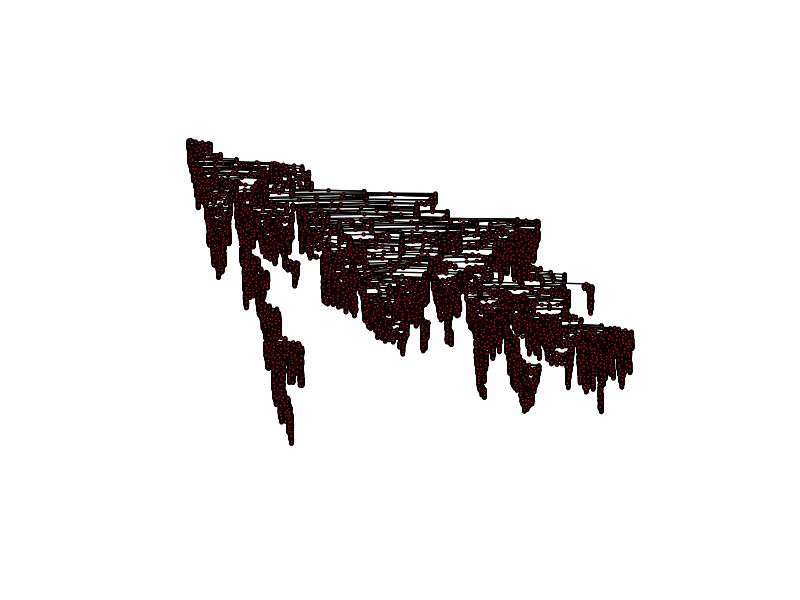
\includegraphics[width=0.75\columnwidth]{renduNX}
\end{center}
	
\paragraph{GraphViz}

\begin{center}
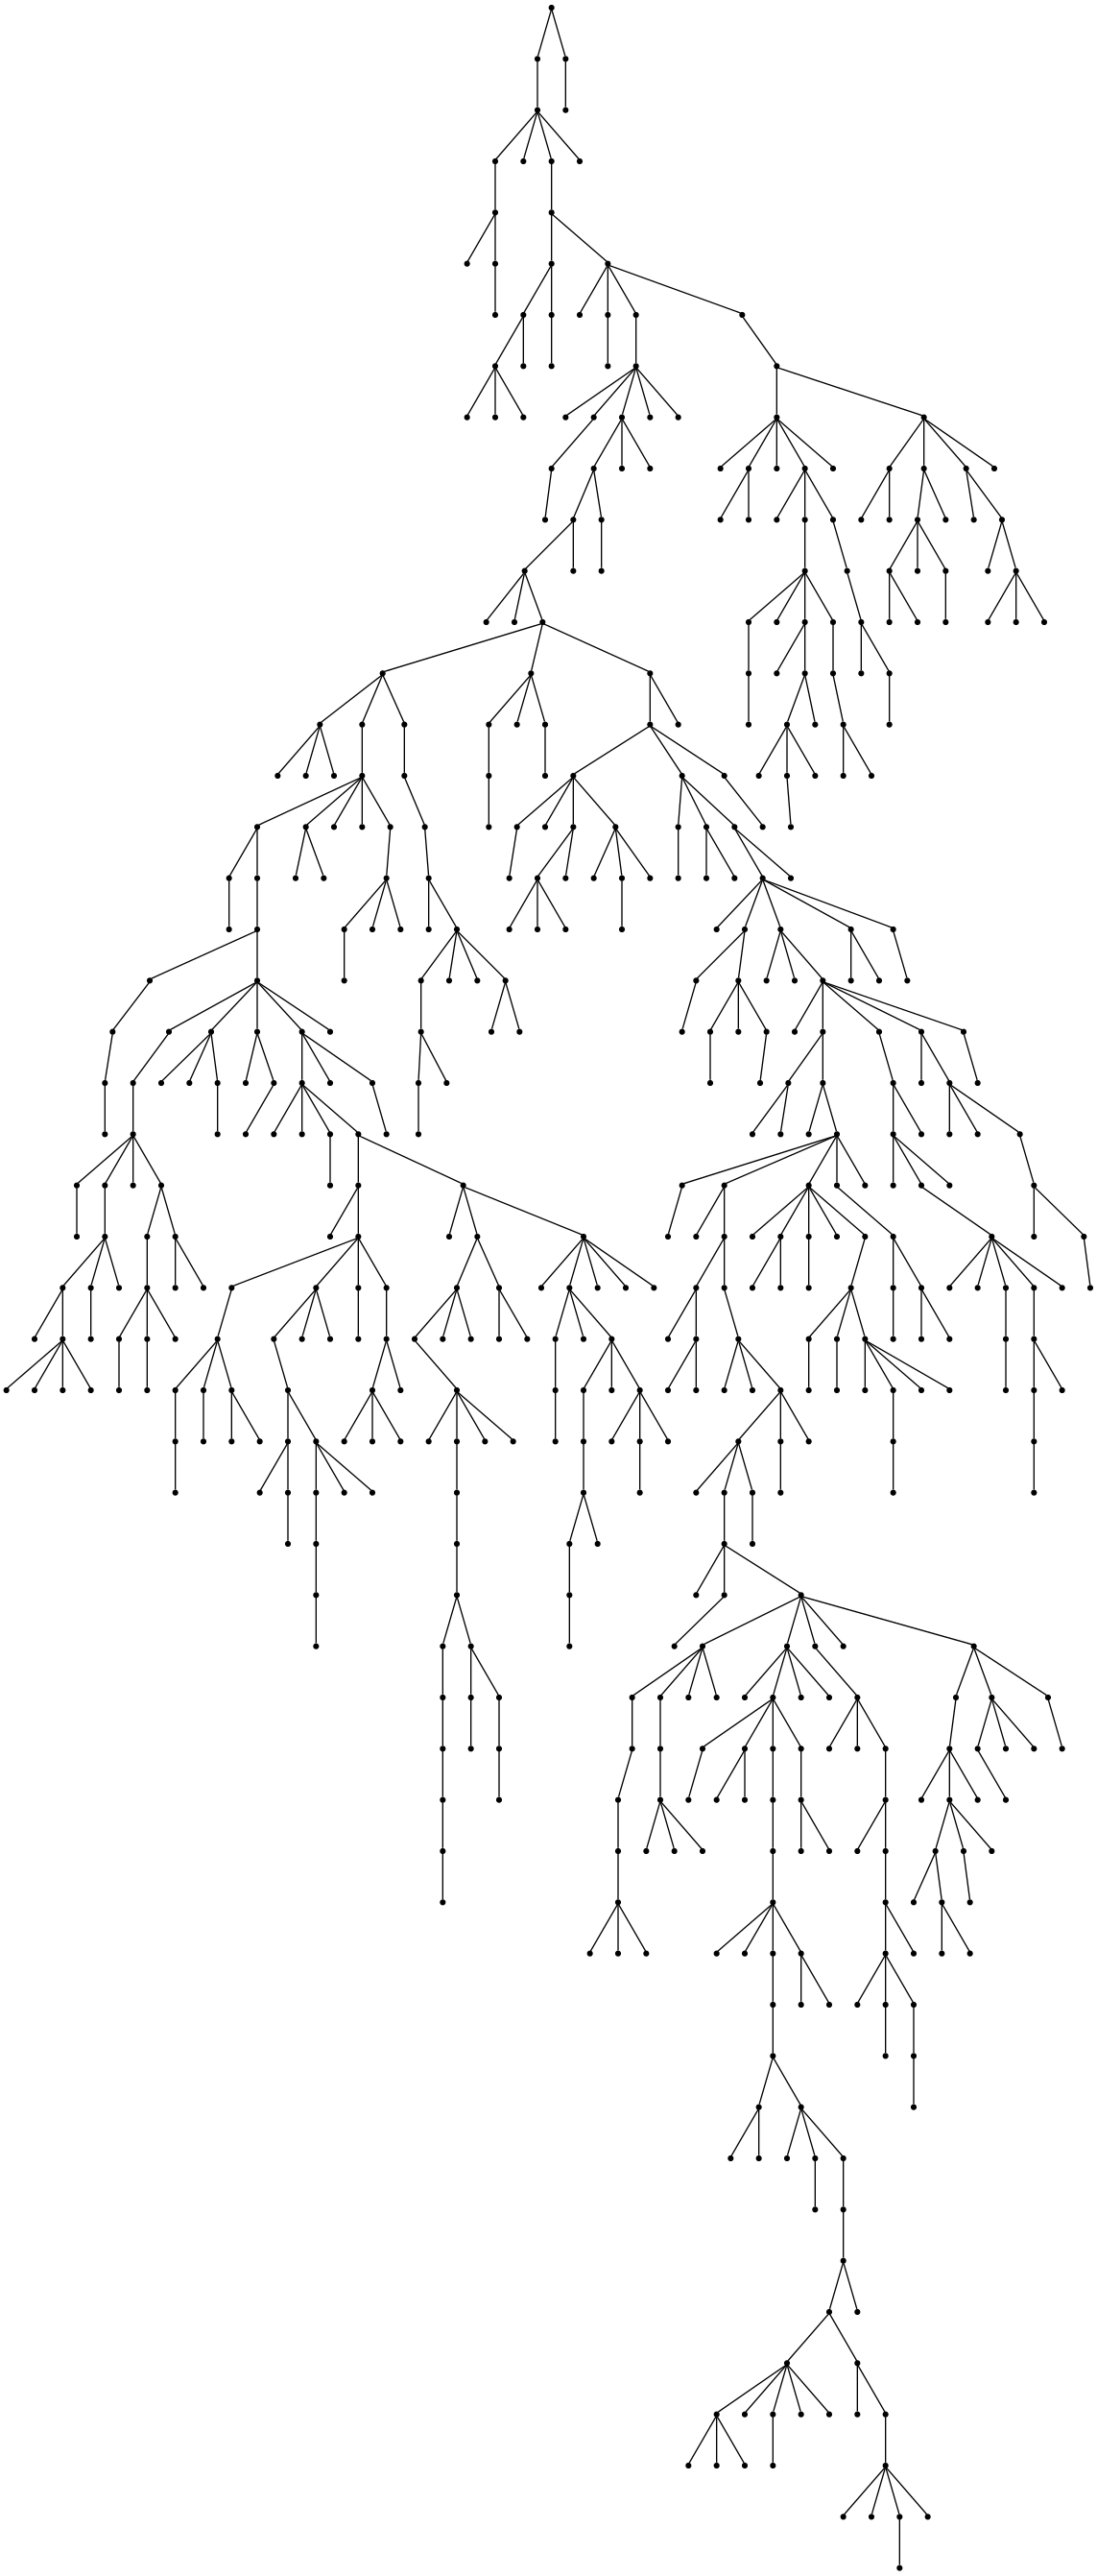
\includegraphics[height=7cm]{renduGV}
\end{center}

%\backmatter
\section{Conclusion}

\begin{frame}
	\frametitle{Bilan}
\end{frame}

\begin{frame}
	\frametitle{Pour la suite}
\end{frame}

%\chapter{Conclusion}
%
%\section{Bilan}
%\paragraph{}L'application \verb|treeDisplay| permet de calculer les coordonnées des n\oe uds d'un arbre en temps linéaire par rapport à ce nombre de n\oe uds. Cependant, l'affichage qui en résulte n'est pas aussi élégant que GraphViz. Nous ne pouvons par exemple pas voir la structure de l'arbre en détail. Mais puisque nous travaillons majoritairement avec des arbres de grande taille, les détails nous intéressent peu. On veut avant tout observer des tendances. 
%\paragraph{} Nous avons également observé que la partie de l'application qui prend le plus de temps à l'exécution est le parsing et la génération de sortie. La clé de la complexité de cette application était donc de lire les fichiers d'entrée et de générer les fichiers de sortie de manière optimale, de façon à utiliser le moins de ressources possible.
%
%\section{Pour la suite}
%
%\paragraph{}La structure choisie permet aussi de représenter des graphes. On peut donc envisager par la suite d'implémenter un algorithme de calcul de coordonnées pour les graphes. Les modules de parsing et de génération sont pleinement réutilisables.
%
%\paragraph{}La complexité en mémoire est actuellement égale à celle en temps. Cependant, on utilisant une table de hachage pour les sous-arbres, on peut devenir sous-linéaire. L'idée consiste à calculer des coordonnées relatives et lorsqu'un arbre comporte deux (ou plus) sous-arbres identiques. Le sous-arbre en question n'est sauvegarder en mémoire qu'une seule fois et la deuxième fois on ne sauvegarde qu'une référence. On calcule ensuite les coordonnées absolues lors de la génération.

%\part{Annexes}
\appendix
\chapter{Images obtenues lors de l'étude préliminaire}

\begin{figure} \centering \resizebox {!}{10cm} {
\begin{tikzpicture}[scale=0.8, every node/.style={scale=0.8}, node distance=1pt]
\input {testTikz500A}
\end{tikzpicture}}
\caption{Arbre linéaire de taille $500$ avec labels obtenu avec TikZ. \label{arbre500TikZA}}
\end{figure}


\begin{figure} \centering \resizebox {!}{10cm} {
\begin{tikzpicture}[scale=0.8, every node/.style={scale=0.8}, node distance=1pt]
\input {testTikz500B}
\end{tikzpicture}}
\caption{Arbre linéaire de taille $500$ sans labels obtenu avec TikZ. \label{arbre500TikZB}}
\end{figure}


\begin{figure} \centering %\resizebox {!}{10cm} {
\input {testAsymptote500A} %}
\caption{Arbre linéaire de taille $500$ avec labels obtenu avec Asymptote. \label{arbre500AsyA}}
\end{figure}


\begin{figure} \centering %\resizebox {!}{10cm} {
\input {testAsymptote500B} %}
\caption{Arbre linéaire de taille $500$ sans labels obtenu avec Asymptote. \label{arbre500AsyB}}
\end{figure}


\begin{figure} \centering %\resizebox {!}{10cm} {
\input {testAsymptote10000A}%}
\caption{Arbre linéaire de taille $10000$ avec labels obtenu avec Asymptote. \label{arbre10000AsyA}}
\end{figure}


\begin{figure} \centering %\resizebox {!}{10cm} {
\input {testAsymptote10000B}%}
\caption{Arbre linéaire de taille $10000$ sans labels obtenu avec Asymptote. \label{arbre10000AsyB}}
\end{figure}

\begin{figure}[h]
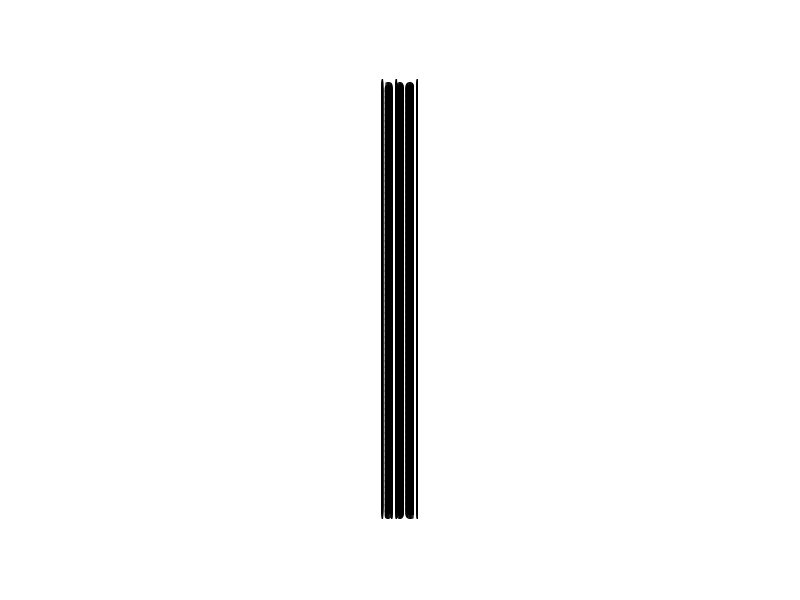
\includegraphics[width=\columnwidth]{testNetworkx500A}
\caption{Arbre linéaire de taille $500$ avec labels obtenu avec NetworkX et Maptplotlib. \label{arbre500NkxA}}
\end{figure}

\begin{figure}[h]
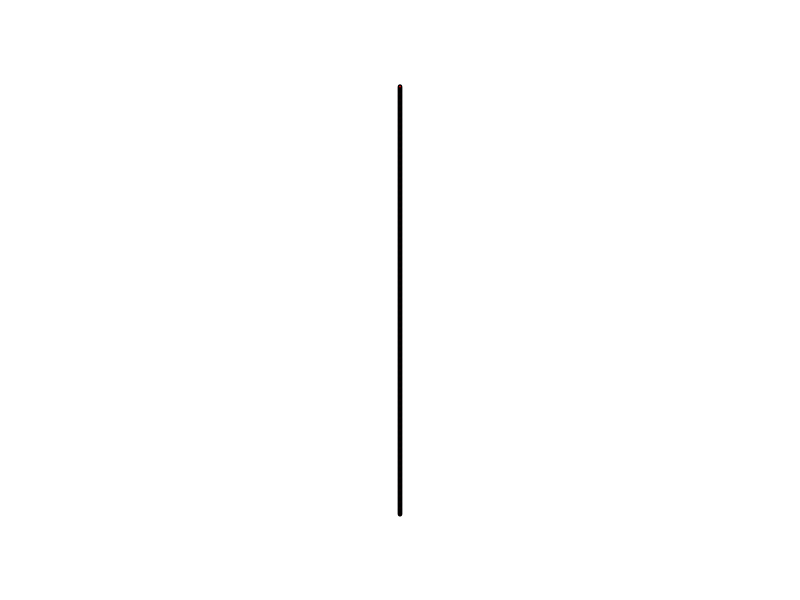
\includegraphics[width=\columnwidth]{testNetworkx500B}
\caption{Arbre linéaire de taille $500$ sans labels obtenu avec NetworkX et Maptplotlib. \label{arbre500NkxB}}
\end{figure}

\begin{figure}[h]
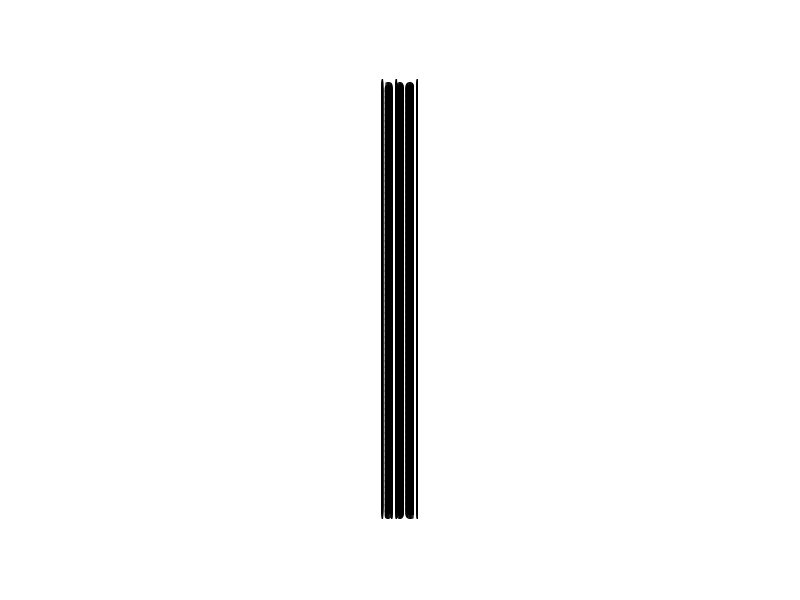
\includegraphics[width=\columnwidth]{testNetworkx500A}
\caption{Arbre linéaire de taille $10000$ avec labels obtenu avec NetworkX et Maptplotlib. \label{arbre10000NkxA}}
\end{figure}

\begin{figure}[h]
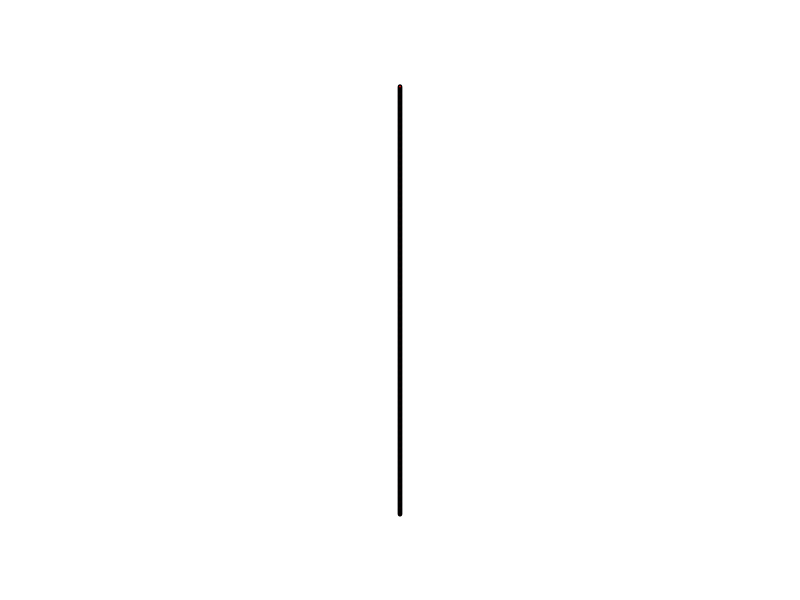
\includegraphics[width=\columnwidth]{testNetworkx500B}
\caption{Arbre linéaire de taille $10000$ sans labels obtenu avec NetworkX et Maptplotlib. \label{arbre10000NkxB}}
\end{figure}

\chapter{Extraits de l'implémentation}

\lstinputlisting[language=Python]{../Src/strParser.py}\label{strParser}
\lstinputlisting[language=Python]{../Src/dotParser.py}\label{dotParser}
\lstinputlisting[language=Python]{../Src/xmlParser.py}\label{xmlParser}

\bibliographystyle{plain-fr}
\nocite{*}
\bibliography{PSTL_biblio}

%\printbibliography


\end{document}
